\documentclass[11pt,a4paper]{article}
\usepackage[utf8]{inputenc}
\usepackage[T1]{fontenc}
\IfFileExists{lmodern.sty}{\usepackage{lmodern}}{}
\usepackage[spanish,es-tabla]{babel}
\usepackage{amsmath,amssymb}
\usepackage{siunitx}
\usepackage{graphicx}
\usepackage{booktabs}
\usepackage{longtable}
\usepackage{caption}
\usepackage{float}
\usepackage[table]{xcolor}
\usepackage[a4paper,margin=2.5cm]{geometry}
\usepackage[hidelinks]{hyperref}
\sisetup{output-decimal-marker={,},group-separator={\,},locale=DE,retain-explicit-plus}
\DeclareSIUnit\microstrain{\text{\ensuremath{\mu\varepsilon}}}
\newcommand{\pend}[1]{\textcolor{red}{\textbf{[PENDIENTE: #1]}}}
\graphicspath{{figures/}}
\setlength{\emergencystretch}{3em}

\title{Determinaci\'on del esfuerzo normal por flexi\'on en una viga instrumentada:\\ soluci\'on anal\'itica, experimental y por elementos finitos}
\author{Brayan Smith Espinosa Villegas \and Samuel Vanegas Correa\\[2pt]
Universidad Pontificia Bolivariana, Medell\'in\\ Elementos Finitos -- Prof.\ Elkin Alonso Taborda Espinosa}
\date{5 de octubre de 2026}

\begin{document}
\maketitle

\begin{abstract}
Se determina el esfuerzo normal por flexi\'on en la posici\'on de una galga extensiom\'etrica adherida a una viga tubular de aluminio 1100 en voladizo, con una carga colgada de \SI{49,77}{N} (pesa de \SI{5}{kg} m\'as tornillo y arandelas, colgados despu\'es de poner la galga en cero). El problema se resuelve de tres formas: con la teor\'ia de vigas de Euler--Bernoulli ($\sigma_{yy}=\SI{11,40}{MPa}$, \SI{165,2}{\microstrain}), con el ensayo de laboratorio ($E\varepsilon=\SI{12,55}{MPa}$, \SI{181,85}{\microstrain}) y con una simulaci\'on por elementos finitos con estudio de malla (Von Mises \SI{11,46}{MPa}; $\sigma_{yy}=\SI{11,44}{MPa}$, tanto en el nodo central como en promedio sobre el \'area de la galga). Tomando el valor anal\'itico como referencia, el $\sigma_{yy}$ del FEM difiere \SI{+0,4}{\percent} y el ensayo \SI{+10,1}{\percent}. Los modelos anal\'itico y FEM son coherentes para la geometr\'ia y la carga nominales. La diferencia con el ensayo puede relacionarse con las dimensiones reales de la viga, con la instrumentaci\'on y con simplificaciones del montaje; los datos disponibles no permiten determinar una causa \'unica.
\end{abstract}

\tableofcontents
\newpage

\section{Introducci\'on}
Una galga extensiom\'etrica mide la deformaci\'on unitaria longitudinal de la superficie en la que est\'a adherida, y el esfuerzo se obtiene con la ley de Hooke. En este trabajo se compara ese esfuerzo con el que predicen la mec\'anica de materiales y una simulaci\'on por elementos finitos, para validar los modelos y analizar las fuentes de error. El informe sigue las cuatro partes del enunciado: soluci\'on anal\'itica (Parte~1), resultados experimentales (Parte~2), simulaci\'on FEM con modelo CAD y convergencia de malla (Parte~3) y comparaci\'on con an\'alisis de errores (Parte~4). Los anexos incluyen los datos, el CAD y los archivos del FEM.

\textbf{Convenciones.} Eje $y$ a lo largo de la viga, $x$ en el ancho y $z$ vertical (positivo hacia arriba); unidades mm, N y MPa. El valor de referencia es el esfuerzo normal longitudinal $\sigma_{yy}$ en el centro de la galga, en $y=\SI{205,5}{mm}$ de la cara superior; el esfuerzo de Von Mises se reporta en la Parte~3 porque lo pide el enunciado. La galga se puso en cero con la viga montada y antes de colgar el tornillo y las arandelas, por lo que la carga que registra es la pesa m\'as el herraje, $P=\SI{49,77}{N}$.

\section{Parte 1: soluci\'on anal\'itica del esfuerzo normal por flexi\'on}
\begin{quote}\small\textit{Resumen de la parte.} Se calcula el esfuerzo normal por flexi\'on en la posici\'on de la galga de una viga tubular de aluminio 1100 en voladizo con la teor\'ia de Euler--Bernoulli. Se parte del equilibrio de la pesa y de sus dos cuerdas, se obtienen las reacciones en la mordaza, los diagramas de cortante y momento, y finalmente el esfuerzo y la deformaci\'on en la galga: $\sigma=\SI{11,40}{MPa}$ y $\varepsilon=\SI{165,2}{\microstrain}$.\end{quote}

\subsection{Datos del montaje}
La viga es un tubo rectangular hueco de aluminio 1100 sujeto por una mordaza. Una pesa cuelga de un tornillo cerca del extremo libre y la galga est\'a pegada en la cara superior. Las coordenadas se toman del modelo CAD (\texttt{VIGA\_FEM.step}), con el eje $y$ a lo largo de la viga.

\begin{table}[H]
\centering
\caption{Datos del montaje.}
\begin{tabular}{llr}
\toprule
Par\'ametro & S\'imbolo & Valor \\
\midrule
M\'odulo de elasticidad (aluminio 1100 \cite{asm}) & $E$ & \SI{69}{GPa} \\
Masa de la pesa & $m_p$ & \SI{5,000}{kg} \\
Masa del tornillo y arandelas & $m_a$ & \SI{0,073}{kg} \\
Gravedad & $g$ & \SI{9,81}{m/s^2} \\
Dimensiones exteriores de la secci\'on & $b\times h$ & \SI{70}{mm}$\times$\SI{30}{mm} \\
Espesor de pared & $t$ & \SI{1}{mm} \\
Longitud total & $L$ & \SI{746}{mm} \\
Borde libre de la mordaza & $y_m$ & \SI{141,83}{mm} \\
Centro de la galga (marca de 198 a \SI{213}{mm}) & $y_g$ & \SI{205,5}{mm} \\
Eje del tornillo (punto de carga) & $y_P$ & \SI{711}{mm} \\
\bottomrule
\end{tabular}
\end{table}

\subsection{Hip\'otesis}
\begin{itemize}
\item Teor\'ia de Euler--Bernoulli de flexi\'on de vigas \cite{beer}, material el\'astico lineal, peque\~nas deformaciones y secci\'on prism\'atica.
\item Carga est\'atica. La viga se comporta como voladizo: la mordaza se modela como empotramiento en $y_m$.
\item \textbf{El peso propio de la viga se excluye.} La galga se puso en cero con la viga ya montada, de modo que el ensayo mide \'unicamente el incremento producido por la pesa y el tornillo. Como referencia, el peso propio aportar\'ia $\approx\SI{0,34}{MPa}$ ($\approx\SI{3}{\percent}$) en la posici\'on de la galga; ese valor ya est\'a dentro del cero y no se suma.
\item En la cara superior, que es una superficie libre, se supone un estado aproximadamente uniaxial en la direcci\'on longitudinal $y$, de modo que $\sigma_{yy}=E\,\varepsilon_{yy}$.
\end{itemize}

\subsection{Paso 1: carga y equilibrio de las cuerdas}
La masa total colgada y su peso son
\begin{align}
m &= m_p+m_a = \SI{5,073}{kg},\\
P &= m\,g = 5{,}073\times 9{,}81 = \SI{49,77}{N}.
\end{align}
La pesa cuelga de dos cuerdas sim\'etricas, cada una a $20^\circ$ de la vertical (figura~\ref{fig:cuerdas}). \textbf{La fuerza $F$ de cada cuerda es la que va a lo largo de la cuerda}; su componente vertical es $F\cos20^\circ$ y la horizontal es $F\sin20^\circ$. Las horizontales son iguales y opuestas y se anulan. El equilibrio vertical del nudo es
\begin{equation}
2F\cos20^\circ = P \quad\Longrightarrow\quad F=\frac{P}{2\cos20^\circ}=\frac{49{,}77}{2\times0{,}9397}=\SI{26,48}{N}.
\end{equation}
Cada cuerda aporta en vertical $F\cos20^\circ=\SI{24,88}{N}$, es decir, $P/2$.

\begin{figure}[H]
\centering
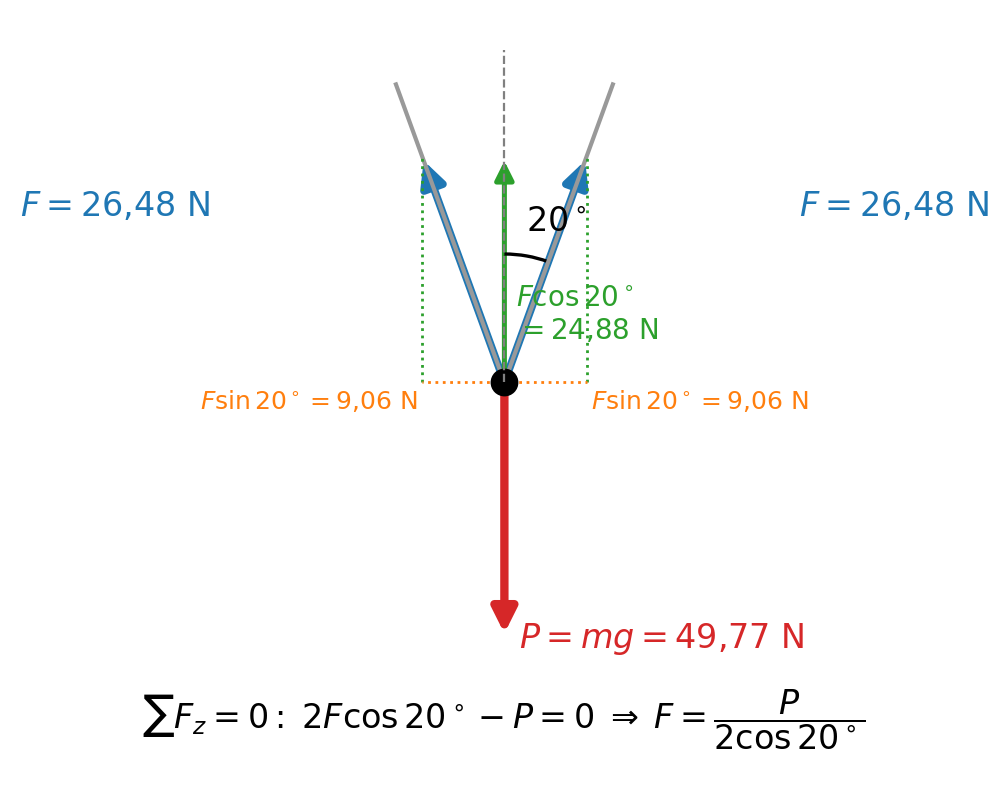
\includegraphics[width=0.72\textwidth]{fig_dcl_cuerdas.png}
\caption{Diagrama de cuerpo libre del nudo de la pesa. Las dos fuerzas $F$ van a lo largo de las cuerdas; sus componentes verticales equilibran el peso.}
\label{fig:cuerdas}
\end{figure}

\paragraph{Comprobaci\'on de consistencia.} Si en un modelo num\'erico se introdujera \SI{24,88}{N} como \emph{magnitud} de cada fuerza inclinada, la componente vertical ser\'ia $24{,}88\cos20^\circ=\SI{23,38}{N}$ y el total vertical \SI{46,76}{N}, es decir, \SI{6}{\percent} menos que el peso. Por eso la magnitud de la fuerza inclinada debe ser \SI{26,48}{N}, o bien deben darse directamente las componentes. Este chequeo (suma de fuerzas verticales $=P$) se verifica tambi\'en en el FEM.

\subsection{Paso 2: diagrama de cuerpo libre de la viga}
Con la carga $P$ aplicada en $y_P$, el empotramiento debe equilibrarla con una reacci\'on vertical y un momento (figura~\ref{fig:dcl}):
\begin{align}
\sum F_z=0 &\;\Rightarrow\; R=P=\SI{49,77}{N},\\
\sum M=0 &\;\Rightarrow\; M_0 = P\,(y_P-y_m)=49{,}77\times(711-141{,}83)=\SI{28,33}{N.m}.
\end{align}

\begin{figure}[H]
\centering
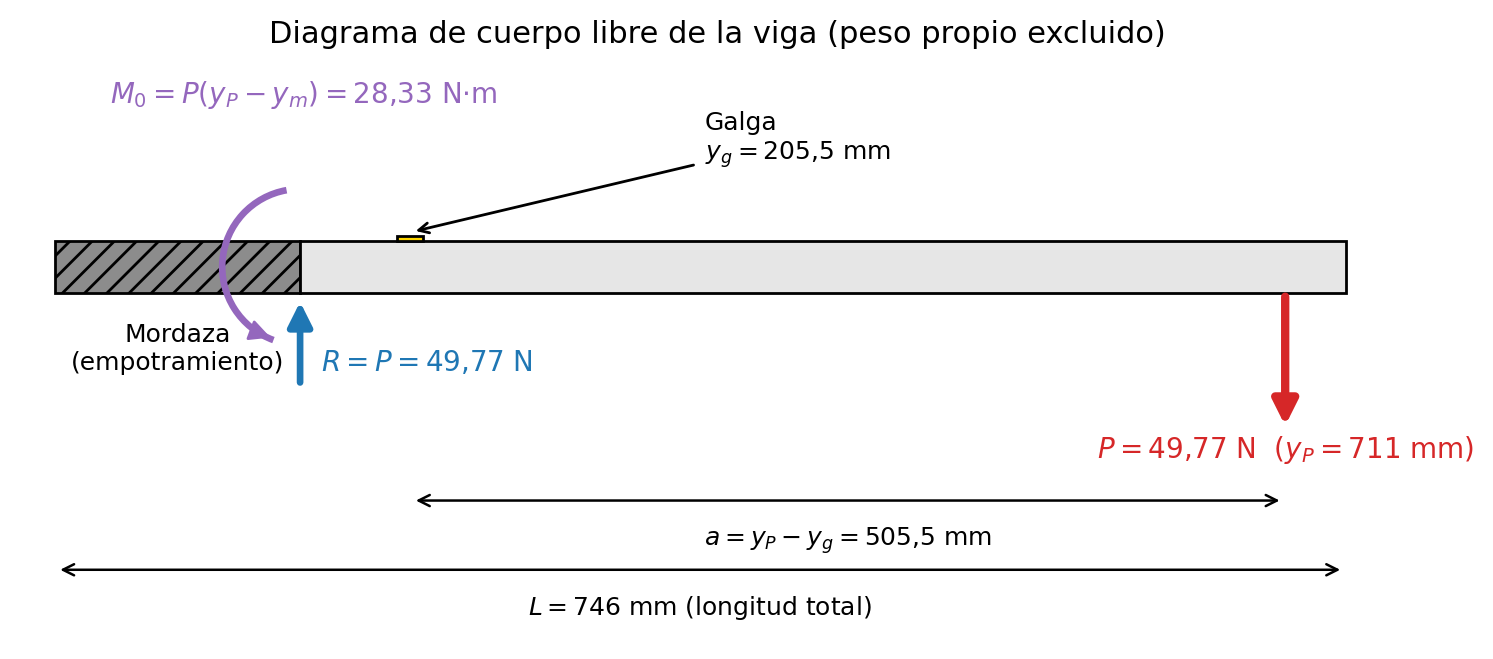
\includegraphics[width=\textwidth]{fig_dcl_viga.png}
\caption{Diagrama de cuerpo libre de la viga, con el peso propio excluido.}
\label{fig:dcl}
\end{figure}

\subsection{Paso 3: fuerzas internas}
Se corta la viga en una posici\'on $y$ entre la mordaza y la carga ($y_m<y<y_P$) y se plantea el equilibrio de la parte libre (a la derecha del corte):
\begin{align}
V(y) &= P = \SI{49,77}{N} \quad (\text{constante}),\\
M(y) &= P\,(y_P-y).
\end{align}
El cortante es constante y el momento decrece linealmente desde $M_0=\SI{28,33}{N.m}$ en la mordaza hasta cero en el punto de carga. Entre $y_P$ y el extremo libre ($y=\SI{746}{mm}$) no hay carga, as\'i que $V=M=0$. Los diagramas aparecen en la figura~\ref{fig:vm}; la galga queda en una zona de momento alto.

\begin{figure}[H]
\centering
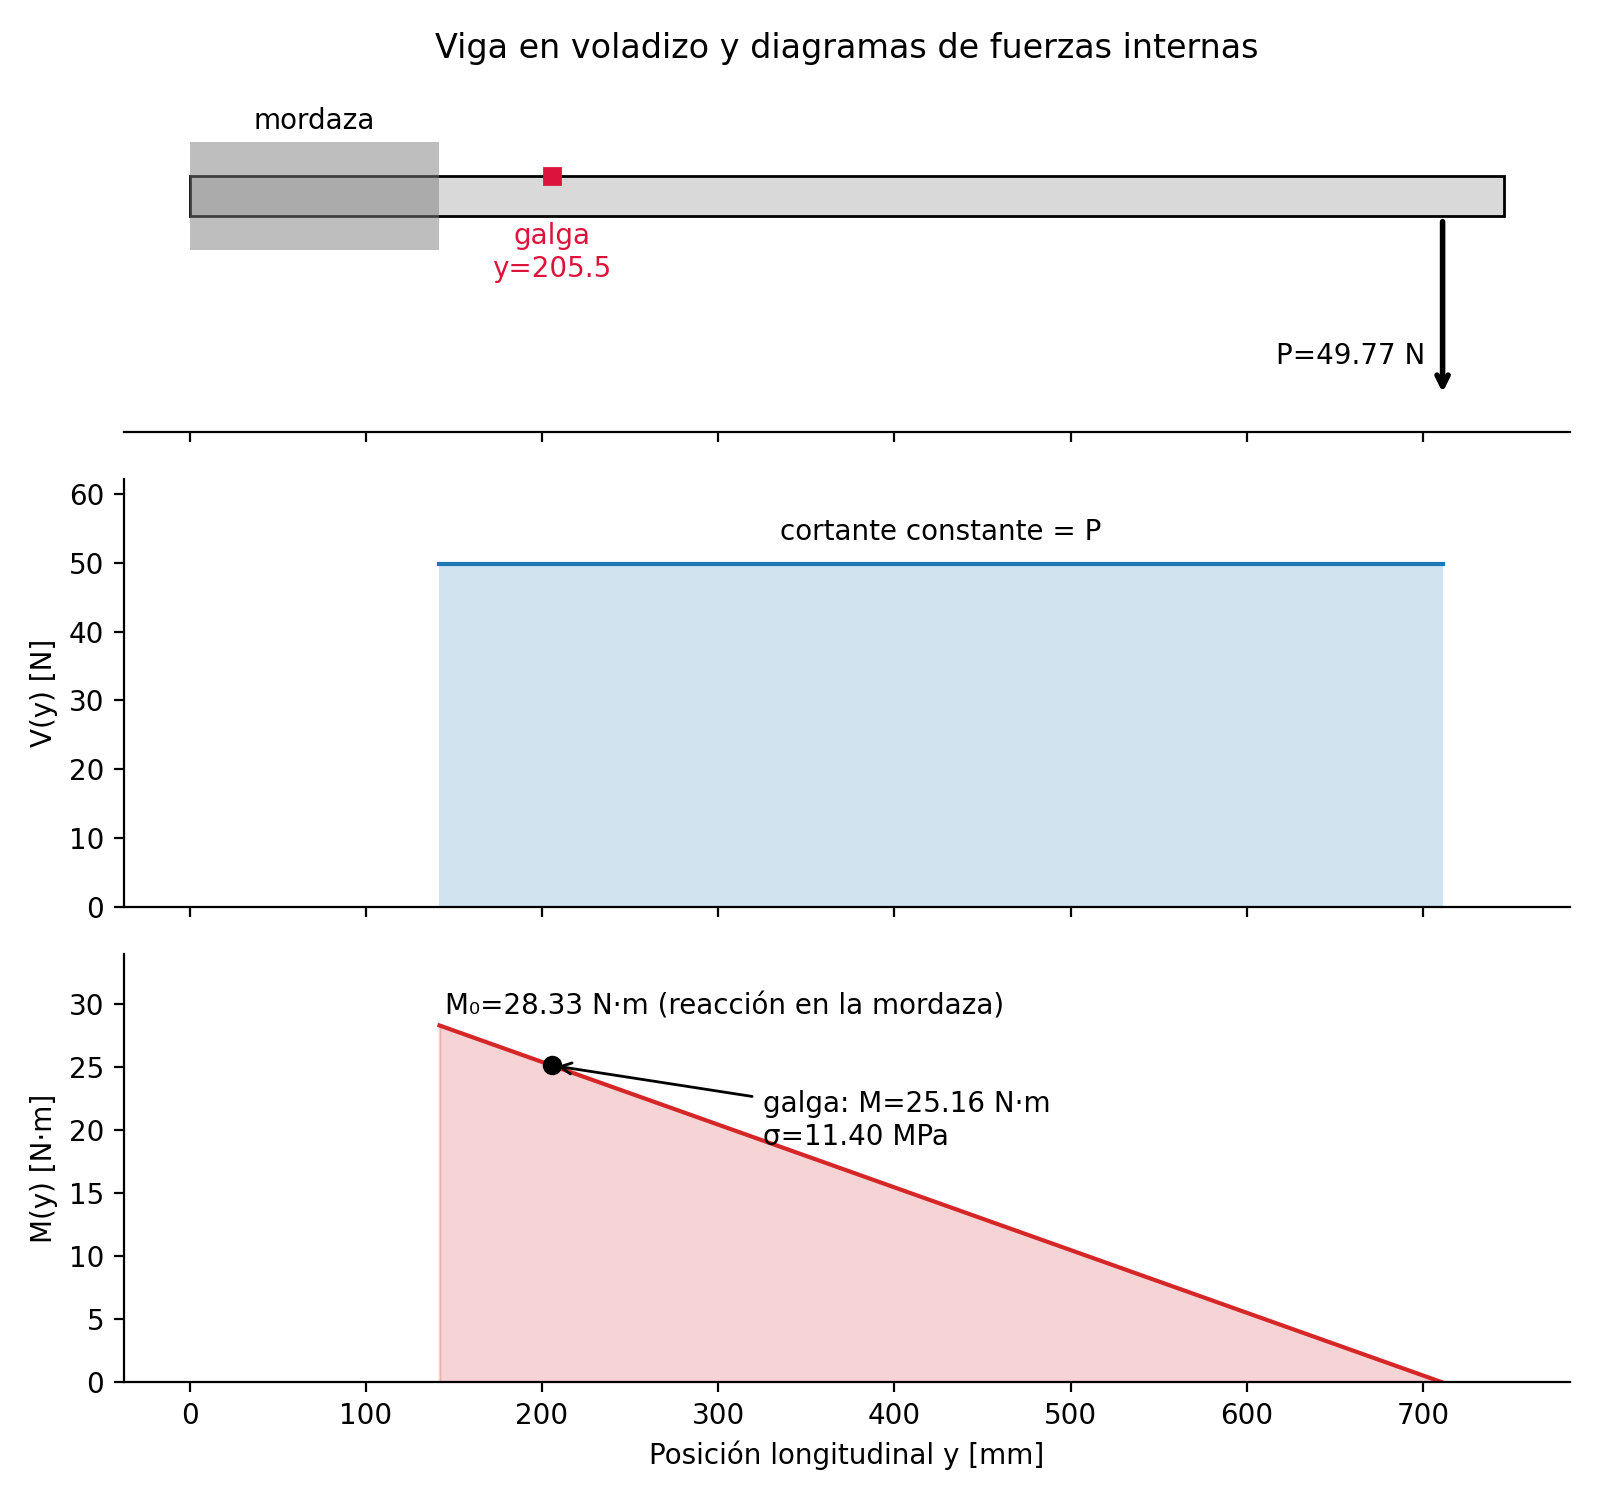
\includegraphics[width=\textwidth]{fig_diagramas_V_M.png}
\caption{Esquema de la viga y diagramas de cortante $V(y)$ y momento flector $M(y)$.}
\label{fig:vm}
\end{figure}

\subsection{Paso 4: propiedades de la secci\'on}
La viga se ensaya con la altura de \SI{30}{mm} en vertical, as\'i que flecta alrededor del eje de menor inercia:
\begin{align}
I &= \frac{b\,h^3-(b-2t)(h-2t)^3}{12}=\frac{70\cdot30^3-68\cdot28^3}{12}=\SI{33105,3}{mm^4},\\
c &= \frac{h}{2}=\SI{15}{mm}.
\end{align}

\subsection{Paso 5: esfuerzo y deformaci\'on en la galga}
El brazo de la carga respecto al centro de la galga y el momento all\'i son
\begin{align}
a &= y_P-y_g = 711-205{,}5=\SI{505,5}{mm},\\
M(y_g) &= P\,a = 49{,}77\times505{,}5=\SI{25156,8}{N.mm}=\SI{25,16}{N.m}.
\end{align}
El esfuerzo normal en la fibra superior y la deformaci\'on correspondiente son
\begin{align}
\sigma_{yy} &= \frac{M\,c}{I}=\frac{25156{,}8\times15}{33105{,}3}=\SI{11,40}{MPa},\\
\varepsilon_{yy} &= \frac{\sigma_{yy}}{E}=\frac{11{,}40}{69000}=\SI{165,2}{\microstrain}.
\end{align}
Como el momento es lineal en $y$, el promedio sobre la rejilla coincide con el valor en su centro. En los extremos de la marca de galga ($y=198$ y \SI{213}{mm}) el esfuerzo vale \SI{11,57}{MPa} y \SI{11,23}{MPa}, es decir, var\'ia \SI{\pm1,5}{\percent} alrededor del centro.

\begin{table}[H]
\centering
\caption{Resumen de la soluci\'on anal\'itica.}
\begin{tabular}{lr}
\toprule
Magnitud & Valor \\
\midrule
Peso $P$ & \SI{49,77}{N} \\
Fuerza en cada cuerda $F$ & \SI{26,48}{N} \\
Reacci\'on $R$ y momento $M_0$ en la mordaza & \SI{49,77}{N}; \SI{28,33}{N.m} \\
Momento en la galga $M(y_g)$ & \SI{25,16}{N.m} \\
Inercia $I$ & \SI{33105,3}{mm^4} \\
Esfuerzo $\sigma_{yy}$ en la galga & \SI{11,40}{MPa} \\
Deformaci\'on $\varepsilon_{yy}$ en la galga & \SI{165,2}{\microstrain} \\
\bottomrule
\end{tabular}
\end{table}

\paragraph{Estado del cero.} El profesor confirm\'o que la galga se puso en cero antes de colgar el tornillo y las arandelas, de modo que la galga registra el efecto de la pesa m\'as el herraje: la carga de comparaci\'on es $P=\SI{49,77}{N}$.

\section{Parte 2: resultados experimentales}
\begin{quote}\small\textit{Resumen de la parte.} Se procesa el archivo del ensayo (\texttt{Viga4SamuelBrayan.csv}) para obtener la deformaci\'on promedio en la galga cuando la carga $P$ est\'a aplicada y el esfuerzo normal asociado. El promedio en la meseta de carga es \SI{185,31}{\microstrain}; al restar la l\'inea base previa a la carga (\SI{3,46}{\microstrain}) la deformaci\'on neta es \SI{181,85}{\microstrain}, que equivale a un esfuerzo de $\sigma=E\varepsilon=\SI{12,55}{MPa}$. Comparado con el valor anal\'itico (\SI{11,40}{MPa}), el resultado es \SI{10,1}{\percent} mayor.\end{quote}

\subsection{Paso 1: explorar el archivo}
El archivo es un CSV con separador \texttt{;} y una sola hoja de datos con dos columnas:
\begin{itemize}
\item \textbf{Time}: marca de tiempo (fecha y hora con milisegundos); se convierte a segundos desde la primera muestra.
\item \textbf{cDAQ1Mod2/ai0}: se\~nal del canal de la galga. Se interpreta como deformaci\'on adimensional (m/m) y se multiplica por $10^{6}$ para expresarla en microdeformaci\'on ($\mu\varepsilon$). El profesor confirm\'o que el archivo ya viene en deformaci\'on.
\end{itemize}

\begin{table}[H]
\centering
\caption{Caracter\'isticas del archivo.}
\begin{tabular}{lr}
\toprule
Muestras & 7\,744 \\
Paso de tiempo & \SI{0,01}{s} (\SI{100}{Hz}) \\
Duraci\'on & \SI{77,43}{s} \\
Deformaci\'on m\'axima registrada (pico transitorio) & \SI{287,5}{\microstrain} \\
\bottomrule
\end{tabular}
\end{table}

\subsection{Paso 2: leer la se\~nal}
La figura~\ref{fig:senal} muestra la deformaci\'on en el tiempo. Se distinguen cinco etapas:
\begin{enumerate}
\item \textbf{Reposo} (0--17 s): la se\~nal est\'a cerca de cero, con una peque\~na deriva hasta \SI{3,5}{\microstrain}.
\item \textbf{Rampa de carga} (17--24 s): al colgar la pesa la se\~nal sube y oscila (vibraci\'on de la viga) hasta estabilizarse.
\item \textbf{Carga $P$ aplicada} (24--55 s): la se\~nal queda en una \emph{meseta} estable, que es la condici\'on que interesa.
\item \textbf{Descarga} (55--58 s): se retira la pesa y la se\~nal cae.
\item \textbf{Reposo final}: vuelve cerca de cero (\SI{1,3}{\microstrain} en promedio entre 66 y 77 s).
\end{enumerate}

\begin{figure}[H]
\centering
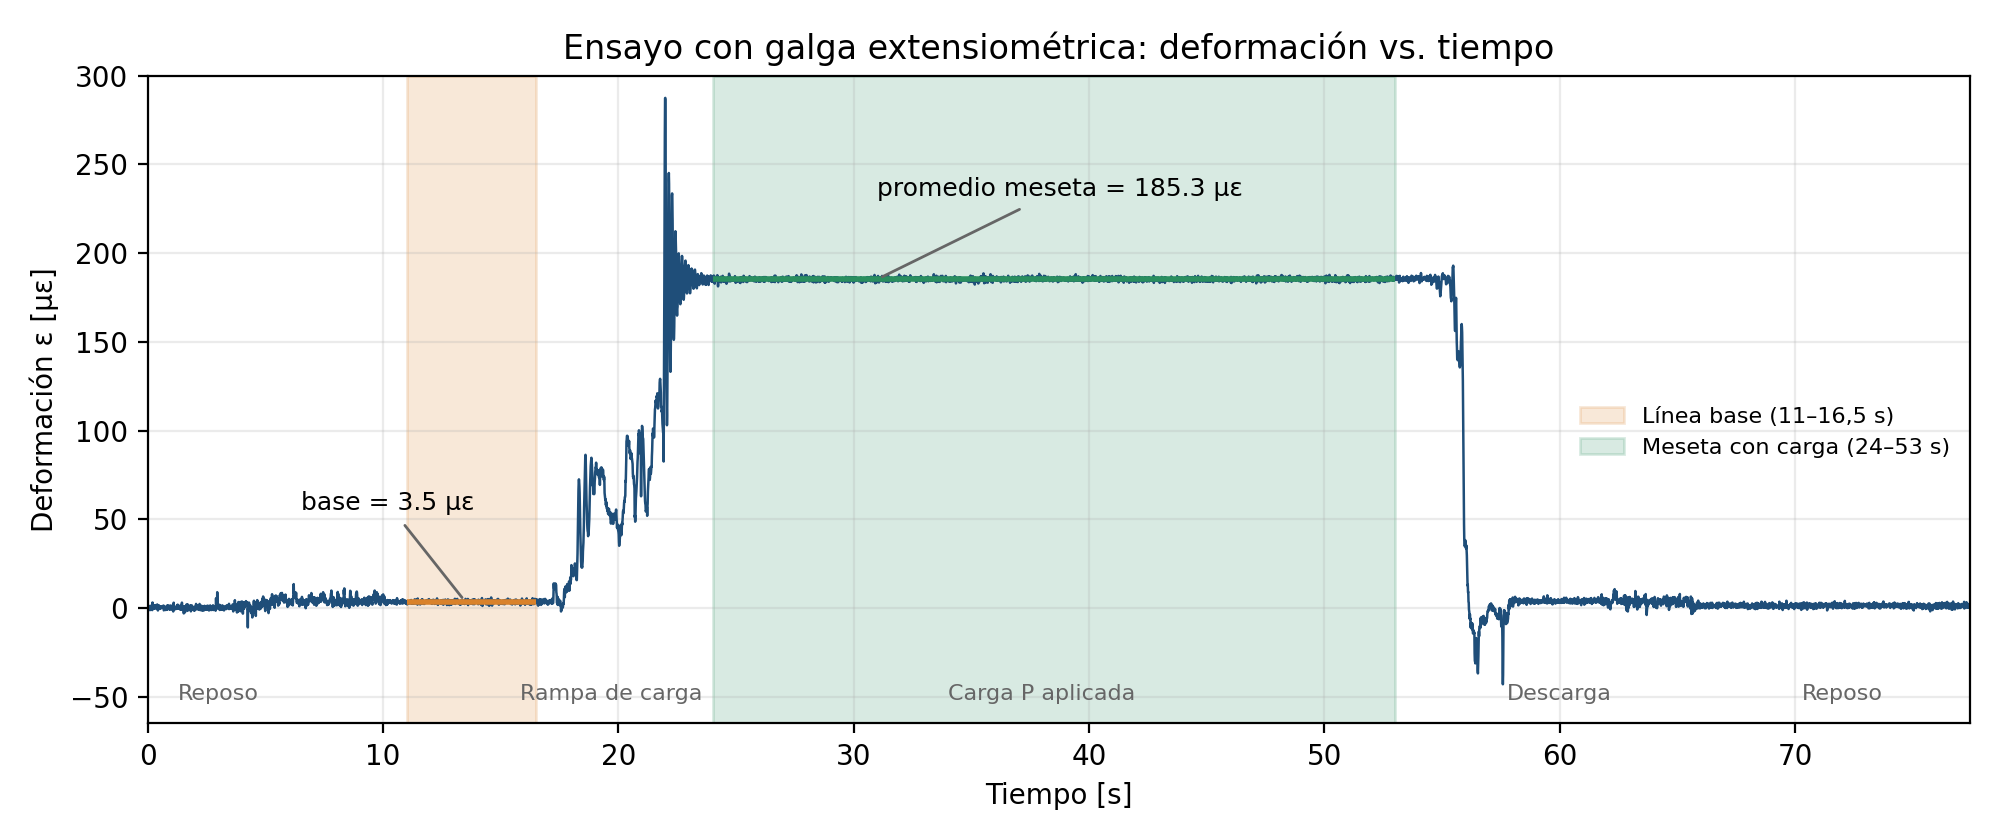
\includegraphics[width=\textwidth]{fig_exp_senal.png}
\caption{Deformaci\'on medida por la galga en el ensayo, con las ventanas usadas para la l\'inea base y para la meseta de carga.}
\label{fig:senal}
\end{figure}

\subsection{Paso 3: deformaci\'on promedio con la carga aplicada}
\paragraph{Ventana de promediado.} Se toma la meseta entre $t=\SI{24}{s}$ y $t=\SI{53}{s}$ ($n=2\,901$ muestras). El l\'imite inferior deja fuera la rampa y la vibraci\'on inicial, y el superior queda antes del inicio de la descarga. La figura~\ref{fig:meseta} muestra que, dentro de esa ventana, la se\~nal es estable y sus valores se distribuyen de forma aproximadamente normal.

\begin{figure}[H]
\centering
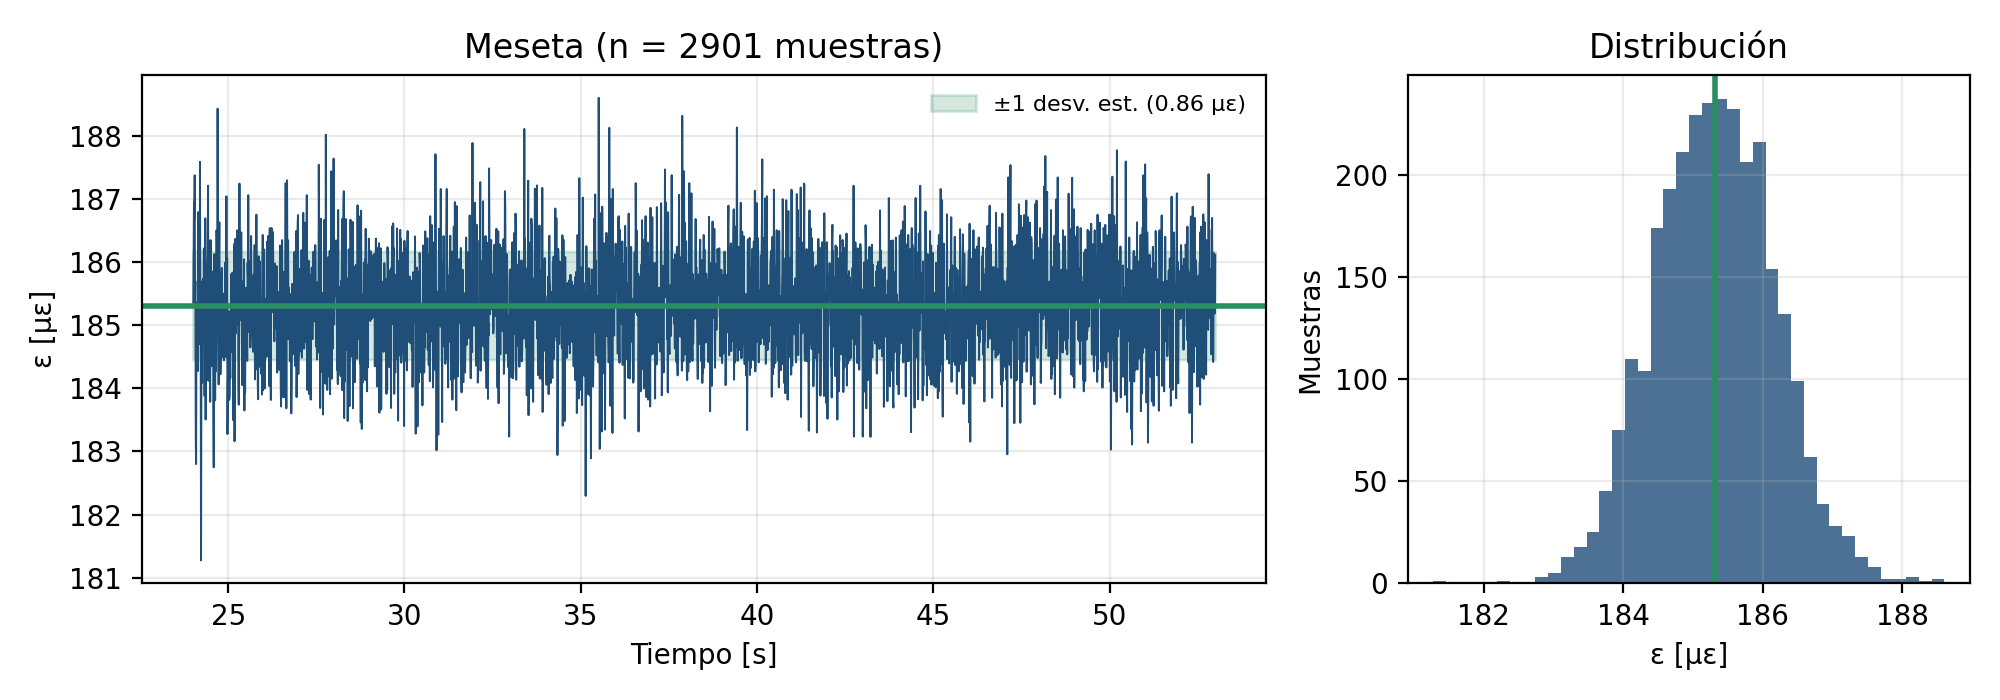
\includegraphics[width=\textwidth]{fig_exp_meseta.png}
\caption{Meseta de carga: se\~nal, promedio (l\'inea verde) y distribuci\'on de las muestras.}
\label{fig:meseta}
\end{figure}

\paragraph{L\'inea base.} La se\~nal no regresa exactamente a cero: antes de cargar vale \SI{3,46}{\microstrain} (promedio entre 11 y \SI{16,5}{s}, $n=551$), mientras que al inicio era \SI{0,39}{\microstrain} (0--3~s) y al final \SI{1,31}{\microstrain} (66--77~s). Se resta la l\'inea base inmediatamente anterior a la carga para referir la medici\'on al estado justo antes de colgar la pesa. Restar una base fija corrige ese desplazamiento de referencia, pero no demuestra que toda deriva durante la meseta est\'e corregida:
\begin{equation}
\varepsilon_{\text{neta}}=\varepsilon_{\text{meseta}}-\varepsilon_{\text{base}}=185{,}31-3{,}46=\SI{181,85}{\microstrain}.
\end{equation}

\paragraph{Sensibilidad a la ventana.} Si se cambia la ventana de la meseta (por ejemplo 26--52~s, 25--50~s o 30--50~s) el promedio var\'ia menos de \SI{0,03}{\microstrain}: la elecci\'on de la ventana no afecta el resultado. La dispersi\'on de las muestras individuales es $s=\SI{0,86}{\microstrain}$. Si las muestras fueran independientes, la incertidumbre estad\'istica de la media ser\'ia $s/\sqrt{n}=\SI{0,016}{\microstrain}$ (y \SI{0,038}{\microstrain} para la diferencia meseta--base); sin embargo, la se\~nal tiene correlaci\'on temporal (autocorrelaci\'on $\approx0{,}29$ a \SI{0,1}{s} y $\approx0{,}23$ a \SI{1}{s}), de modo que ese valor subestima la incertidumbre de la media \cite{gum}. Ninguno de estos n\'umeros es la incertidumbre total del ensayo, que debe incluir el cero, la calibraci\'on, el factor de galga, el puente, $E$ y la repetibilidad entre ensayos; esa evaluaci\'on queda pendiente.

\subsection{Paso 4: esfuerzo en la galga}
Con $E=\SI{69}{GPa}$ y suponiendo estado aproximadamente uniaxial en la cara superior (direcci\'on longitudinal $y$; el FEM de la Parte~3 muestra que las dem\'as componentes del esfuerzo en la galga son menores que el \SI{0,4}{\percent} de $\sigma_{yy}$), la ley de Hooke da
\begin{equation}
\sigma_{yy}=E\,\varepsilon_{\text{neta}}=69\,000\times181{,}85\times10^{-6}=\SI{12,55}{MPa}.
\end{equation}

\begin{table}[H]
\centering
\caption{Resultados experimentales en la galga.}
\begin{tabular}{lrr}
\toprule
 & Sin l\'inea base & Con l\'inea base \\
\midrule
Deformaci\'on promedio en la meseta & \SI{185,31}{\microstrain} & \SI{181,85}{\microstrain} \\
Desviaci\'on est\'andar de la meseta & \multicolumn{2}{c}{\SI{0,86}{\microstrain}} \\
Esfuerzo $\sigma=E\varepsilon$ & \SI{12,79}{MPa} & \SI{12,55}{MPa} \\
\bottomrule
\end{tabular}
\end{table}

El valor medido que se adopta es el de la columna \emph{con l\'inea base}: \textbf{$\varepsilon=\SI{181,85}{\microstrain}$ y $\sigma=\SI{12,55}{MPa}$}.

\subsection{Paso 5: carga que corresponde a esa medici\'on}
La galga se puso en cero con la viga montada y \emph{antes} de colgar el tornillo y las arandelas (confirmado por el profesor). Por eso la galga registra el efecto de la pesa m\'as el herraje, y la carga de comparaci\'on es la de la Parte~1: $P=(5{,}000+0{,}073)\times9{,}81=\SI{49,77}{N}$.

\begin{table}[H]
\centering
\caption{Comparaci\'on preliminar con la teor\'ia.}
\begin{tabular}{lr}
\toprule
Carga que registra la galga & \SI{49,77}{N} \\
Esfuerzo te\'orico (Parte~1) & \SI{11,40}{MPa} \\
Deformaci\'on te\'orica & \SI{165,2}{\microstrain} \\
Esfuerzo medido (con l\'inea base) & \SI{12,55}{MPa} \\
\textbf{Diferencia medido vs.\ te\'orico} & \textbf{\SI{+10,1}{\percent}} \\
Diferencia sin restar la l\'inea base & \SI{+12,2}{\percent} \\
\bottomrule
\end{tabular}
\end{table}

El esfuerzo medido es \SI{10,1}{\percent} mayor que el te\'orico. Si el herraje hubiera estado colgado al poner el cero, la carga ser\'ia solo la pesa (\SI{49,05}{N}) y la diferencia subir\'ia a \SI{11,7}{\percent}; con la confirmaci\'on del profesor ese caso queda descartado.

\subsection{Paso 6: cadena de medici\'on y factores propios de la galga}
\subsubsection{Equipo de adquisici\'on}
El ensayo se adquiri\'o con un chasis NI cDAQ-9174 que aloja un m\'odulo NI~9237 (entrada de puente para galgas, 4 canales, 24~bits y \SI{50}{kS/s} por canal) y un m\'odulo NI~9215 (entrada de voltaje $\pm\SI{10}{V}$, 16~bits) \cite{ni9237,ni9215}. El canal del archivo, \texttt{cDAQ1Mod2/ai0}, corresponde al m\'odulo de la ranura~2.

El NI~9237 no mide deformaci\'on directamente: mide el desbalance del puente de Wheatstone, y la deformaci\'on se calcula por software a partir de la configuraci\'on del canal (factor de galga, tipo de puente, tensi\'on de excitaci\'on y cero inicial) \cite{ni9237}. El profesor confirm\'o que el canal exportado ya est\'a en deformaci\'on adimensional, as\'i que no se requiere conversi\'on adicional.

\subsubsection{Efecto del factor de galga}
Si el factor de galga escrito en el programa ($GF_\text{conf}$) difiere del real de la galga pegada ($GF_\text{real}$), la deformaci\'on registrada queda escalada:
\begin{equation}
\varepsilon_\text{real}=\varepsilon_\text{medida}\,\frac{GF_\text{conf}}{GF_\text{real}}.
\end{equation}
El principio de la galga (resistencia que var\'ia con la deformaci\'on seg\'un el factor de galga) se describe en \cite{hoff}. Las galgas de l\'amina met\'alica tienen t\'ipicamente factores cercanos a 2 (del orden de 2,0 a 2,1), de modo que una diferencia de pocos por ciento entre el valor configurado y el real es plausible. La tabla~\ref{tab:gf} muestra c\'omo cambiar\'ia el esfuerzo medido y su diferencia con la teor\'ia (\SI{11,40}{MPa}).

\begin{table}[H]
\centering
\caption{Sensibilidad del resultado experimental al factor de galga.}
\label{tab:gf}
\begin{tabular}{rrrr}
\toprule
$GF_\text{conf}/GF_\text{real}$ & $\varepsilon_\text{real}$ & $\sigma$ & Diferencia vs.\ teor\'ia \\
\midrule
0,95 & \SI{172,8}{\microstrain} & \SI{11,92}{MPa} & \SI{+4,6}{\percent} \\
0,97 & \SI{176,4}{\microstrain} & \SI{12,17}{MPa} & \SI{+6,8}{\percent} \\
1,00 & \SI{181,9}{\microstrain} & \SI{12,55}{MPa} & \SI{+10,1}{\percent} \\
1,03 & \SI{187,3}{\microstrain} & \SI{12,92}{MPa} & \SI{+13,4}{\percent} \\
1,05 & \SI{190,9}{\microstrain} & \SI{13,18}{MPa} & \SI{+15,6}{\percent} \\
\bottomrule
\end{tabular}
\end{table}

Es un an\'alisis de sensibilidad. El profesor indic\'o que el efecto del factor de galga es peque\~no; no se cuantific\'o en este trabajo y se mantiene en la Parte~4 como una de las causas posibles de la diferencia.

\subsubsection{Otros factores de la galga y de la adquisici\'on}
Los factores del modelo (espesor real, m\'odulo de elasticidad, dimensiones y carga) se discuten en la Parte~4, junto con el FEM.
\begin{itemize}
\item \textbf{Cero y deriva.} La l\'inea base var\'ia entre \SI{0,4}{} y \SI{3,5}{\microstrain} a lo largo del registro; restar la base previa corrige el desplazamiento de referencia, pero la deriva residual durante la meseta no est\'a cuantificada.
\item \textbf{Tipo de puente y cables.} El resultado depende de que la configuraci\'on del canal (cuarto o medio puente, resistencia nominal, excitaci\'on) coincida con el cableado real. No se dispone de esa configuraci\'on; se mantiene como causa posible.
\item \textbf{Posici\'on de la galga.} Si el centro real est\'a desplazado \SI{10}{mm} respecto a \SI{205,5}{mm}, el esfuerzo te\'orico cambia $\approx\SI{2}{\percent}$, porque el momento var\'ia linealmente con $y$.
\item \textbf{Orientaci\'on.} Una galga mal alineada con el eje $y$ mide menos deformaci\'on longitudinal, no m\'as; por s\'i sola no explica una lectura alta.
\item \textbf{Estado uniaxial.} $\sigma=E\varepsilon$ supone esfuerzo uniaxial. Una cara libre no lo garantiza por s\'i sola; aqu\'i lo respalda el tensor de esfuerzos del FEM en la galga (Parte~3), cuyas componentes distintas de $\sigma_{yy}$ son muy peque\~nas.
\end{itemize}

\section{Parte 3: simulaci\'on por elementos finitos}
\begin{quote}\small\textit{Resumen de la parte.} Se modela la viga tubular instrumentada en CAD con la orientaci\'on del ensayo y se resuelve por elementos finitos (tetraedros parab\'olicos, CalculiX). Se estudian cinco tama\~nos de malla (25, 20, 15, 10 y \SI{5}{mm}), m\'as dos de control (7 y \SI{4}{mm}): entre las mallas de 10 a \SI{4}{mm} el esfuerzo en la galga var\'ia menos de \SI{0,1}{\percent}. Con la malla de \SI{5}{mm}, el esfuerzo de Von Mises en la galga es \SI{11,46}{MPa}, tanto en el nodo central como en promedio sobre el \'area de la galga; el esfuerzo normal longitudinal es $\sigma_{yy}=\SI{11,44}{MPa}$, \SI{0,4}{\percent} por encima del valor anal\'itico (\SI{11,40}{MPa}), y el equilibrio de reacciones reproduce la carga aplicada (\SI{49,77}{N}).\end{quote}

\subsection{Modelo CAD}
\subsubsection{Geometr\'ia y orientaci\'on del ensayo}
El modelo se construy\'o en Autodesk Fusion y se export\'o en formato neutro STEP (\texttt{VIGA\_FEM.step}). Reproduce el montaje del ensayo: la viga es un tubo rectangular hueco de aluminio 1100 de $70\times30$~mm con pared de \SI{1}{mm} y \SI{746}{mm} de longitud, en voladizo, con el lado largo de la secci\'on (\SI{70}{mm}) en horizontal y la altura de \SI{30}{mm} en vertical. El eje $y$ va a lo largo de la viga, el eje $x$ es el ancho y el eje $z$ es vertical (positivo hacia arriba). La galga est\'a en la cara superior ($z=\SI{30}{mm}$).

El modelo contiene siete s\'olidos (figura~\ref{fig:cad}):
\begin{itemize}
\item tres tramos de viga: el tramo de $y=0$ a \SI{140}{mm} y el de \SI{140}{} a \SI{141,83}{mm} (zona de la mordaza) y el tramo libre de \SI{141,83}{} a \SI{746}{mm};
\item un tornillo, dos arandelas y una tuerca de cierre idealizada, que sujetan las cuerdas de la pesa en $y=\SI{711}{mm}$ (agujero pasante de \SI{8}{mm}).
\end{itemize}
La marca de la galga es un rect\'angulo de $5\times15$~mm en la cara superior, entre $y=198$ y \SI{213}{mm} y entre $x=14{,}07$ y \SI{19,07}{mm}; su centro, donde se lee el esfuerzo, est\'a en $(16{,}57;\,205{,}5;\,30)$~mm.

\begin{figure}[H]
\centering
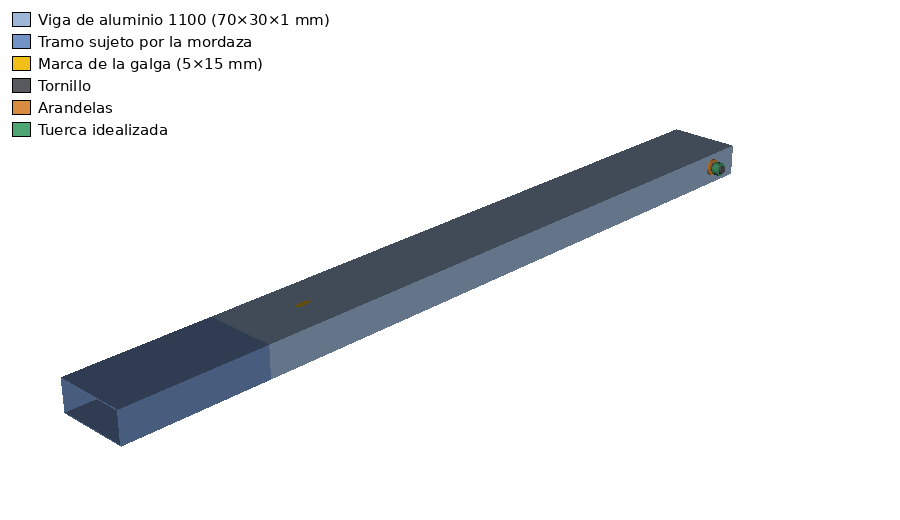
\includegraphics[width=\textwidth]{cad_general.png}
\caption{Modelo CAD en la orientaci\'on del ensayo: viga en voladizo (mordaza a la izquierda), marca de la galga en la cara superior y herraje de carga cerca del extremo libre.}
\label{fig:cad}
\end{figure}

\begin{figure}[H]
\centering
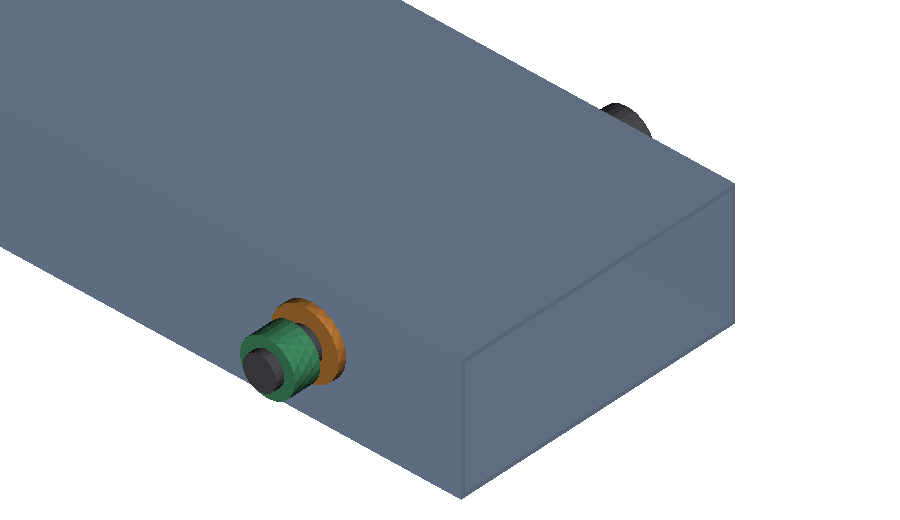
\includegraphics[width=0.62\textwidth]{cad_carga.png}\hfill
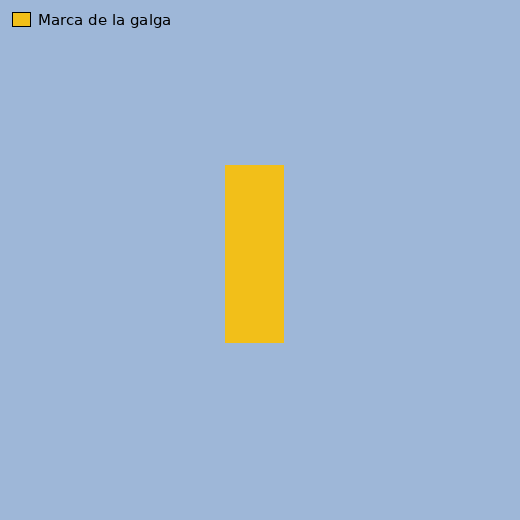
\includegraphics[width=0.33\textwidth]{cad_galga.png}
\caption{Detalles del CAD. Izquierda: tornillo, arandelas y tuerca en el punto de carga ($y=\SI{711}{mm}$). Derecha: vista superior de la marca de la galga (amarillo).}
\label{fig:detalles}
\end{figure}

\subsection{Condiciones de la simulaci\'on}
Se resolvi\'o un an\'alisis est\'atico lineal con el solver CalculiX 2.21 \cite{dhondt}, con la malla generada en gmsh 4.15 \cite{gmsh}. CalculiX es el solver que usa PrePoMax \cite{prepomax}, por lo que el modelo es equivalente al que se montar\'ia en esa interfaz. Las condiciones son:
\begin{itemize}
\item \textbf{Material:} aluminio 1100, $E=\SI{69}{GPa}$, $\nu=0{,}33$ \cite{asm}.
\item \textbf{Elementos:} tetraedros parab\'olicos de 10 nodos (C3D10). Las piezas comparten nodos en sus interfaces (malla conforme), lo que equivale a uniones pegadas entre viga, tornillo, arandelas y tuerca.
\item \textbf{Apoyo:} desplazamientos impedidos en las caras exteriores del tramo de viga dentro de la mordaza ($y\le\SI{141,83}{mm}$).
\item \textbf{Carga:} dos fuerzas de $F=\SI{26,48}{N}$ a $20^\circ$ de la vertical, aplicadas sobre el eje del tornillo en $y=\SI{711}{mm}$ y repartidas en los tramos visibles del eje mediante un acople r\'igido. Sus componentes son $F_z=-F\cos20^\circ=\SI{-24,88}{N}$ y $F_x=\pm F\sin20^\circ=\SI{\pm9,06}{N}$; las horizontales se anulan y la suma vertical es $\SI{49,77}{N}$ ($5{,}073~\text{kg}\times9{,}81$), igual a la usada en la Parte~1.
\item \textbf{Gravedad:} no se aplica. La galga se puso en cero con la viga montada, de modo que el ensayo solo mide el efecto de la carga a\~nadida; el peso propio (\SI{0,34}{MPa}, $\approx\SI{3}{\percent}$) no entra en la comparaci\'on.
\end{itemize}

\subsection{Convergencia de malla}
Se repiti\'o el c\'alculo con tama\~nos de elemento de 25, 20, 15, 10 y \SI{5}{mm}, y adem\'as de 7 y \SI{4}{mm} como control. El criterio es el habitual: refinar hasta que la magnitud de inter\'es deje de cambiar \cite{cook}. En cada malla se leen, en el centro de la galga, el esfuerzo de Von Mises (pedido por el enunciado) y el esfuerzo normal $\sigma_{yy}$, y el \textbf{promedio sobre el \'area de la galga} (cara de $5\times15$~mm del CAD), descrito m\'as abajo. La variaci\'on se define como $\Delta(h)=|VM(h)-VM_{\SI{4}{mm}}|/VM_{\SI{4}{mm}}$. La figura~\ref{fig:conv} y la tabla~\ref{tab:conv} muestran el resultado, y las figuras~\ref{fig:m25}--\ref{fig:m5} las capturas de cada malla (izquierda: viga completa; derecha: acercamiento a la galga con las aristas de los elementos).

\begin{table}[H]
\centering
\caption{Convergencia del esfuerzo de Von Mises en la galga.}
\label{tab:conv}
\small
\setlength{\tabcolsep}{4pt}
\begin{tabular}{rrrrrrr}
\toprule
Tama\~no & Nodos & Elementos & \multicolumn{2}{c}{Von Mises [MPa]} & \multicolumn{2}{c}{$\sigma_{yy}$ [MPa]} \\
\cmidrule(lr){4-5}\cmidrule(lr){6-7}
[mm] & & & centro & prom.\ \'area & centro & prom.\ \'area \\
\midrule
25 & 10\,416 & 5\,175 & 11,608 & 11,596 & 11,595 & 11,600 \\
20 & 11\,735 & 5\,837 & 11,520 & 11,566 & 11,572 & 11,491 \\
15 & 16\,076 & 7\,999 & 11,536 & 11,557 & 11,498 & 11,466 \\
10 & 28\,263 & 14\,086 & 11,473 & 11,472 & 11,453 & 11,452 \\
7 & 50\,154 & 25\,029 & 11,468 & 11,468 & 11,447 & 11,450 \\
\textbf{5} & \textbf{90\,815} & \textbf{45\,706} & \textbf{11,464} & \textbf{11,463} & \textbf{11,442} & \textbf{11,445} \\
4 & 138\,585 & 69\,809 & 11,467 & 11,466 & 11,452 & 11,453 \\
\bottomrule
\end{tabular}
\end{table}

\begin{figure}[H]
\centering
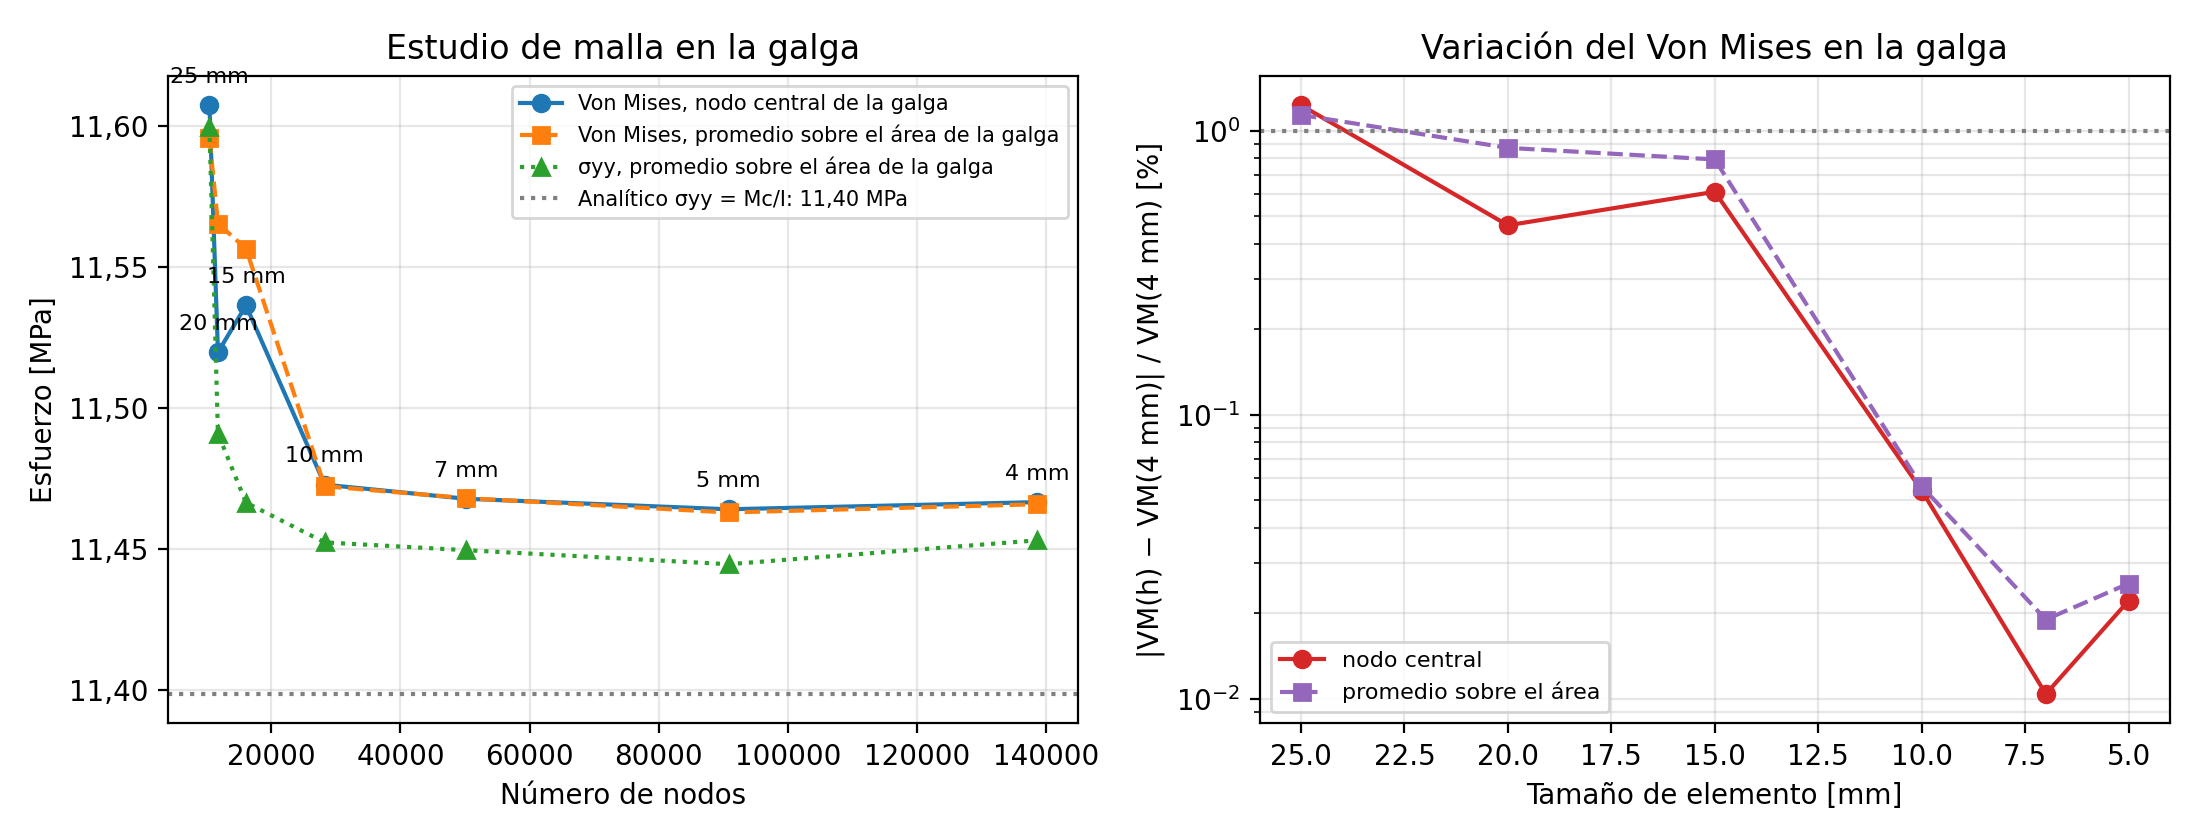
\includegraphics[width=\textwidth]{fig_convergencia_vm.png}
\caption{Estudio de malla: esfuerzo en la galga contra el n\'umero de nodos (izquierda) y variaci\'on $\Delta(h)$ respecto a la malla de \SI{4}{mm} (derecha).}
\label{fig:conv}
\end{figure}

\paragraph{Lectura.} De \SI{25}{} a \SI{10}{mm} el valor de Von Mises baja de \SI{11,61}{} a \SI{11,47}{MPa} ($-\SI{1,2}{\percent}$); entre las mallas de 10 a \SI{4}{mm} la variaci\'on es menor que \SI{0,1}{\percent} (de 10 a \SI{5}{mm}: $-\SI{0,08}{\percent}$ en Von Mises y $-\SI{0,09}{\percent}$ en $\sigma_{yy}$) y el valor queda entre \SI{11,46}{} y \SI{11,47}{MPa}. Hay, por tanto, evidencia de estabilizaci\'on local del resultado en esta familia de mallas, y se toma la de \SI{5}{mm} (\SI{90815}{} nodos) como resultado. La serie no es mon\'otona, as\'i que no se usa para extrapolar un valor exacto, y la variaci\'on entre mallas no es una cota demostrada del error de discretizaci\'on.

\paragraph{Por qu\'e se mide en la galga y no el m\'aximo global.} El m\'aximo de Von Mises sobre todo el modelo crece al refinar (\SI{18,3}{}, \SI{19,3}{}, \SI{20,3}{}, \SI{25,7}{} y \SI{26,9}{MPa} de 25 a \SI{5}{mm}, y \SI{36,8}{MPa} con la malla de control de \SI{4}{mm}). En todas las mallas est\'a en el borde de la zona fija de la mordaza ($y\approx\SI{141}{mm}$, caras superior e inferior), justo donde termina la restricci\'on de desplazamiento; en la malla de \SI{5}{mm}, en $(-15{,}43;\,140{,}92;\,30)$~mm. Ese valor depende de c\'omo se idealiza el apoyo y del tama\~no de los elementos, de modo que no es un resultado f\'isico fiable ni lo que mide la galga, y no sirve para caracterizar una falla. Por eso la convergencia se verifica en el punto de la galga, que est\'a en una zona de esfuerzo suave.

\begin{figure}[H]\centering
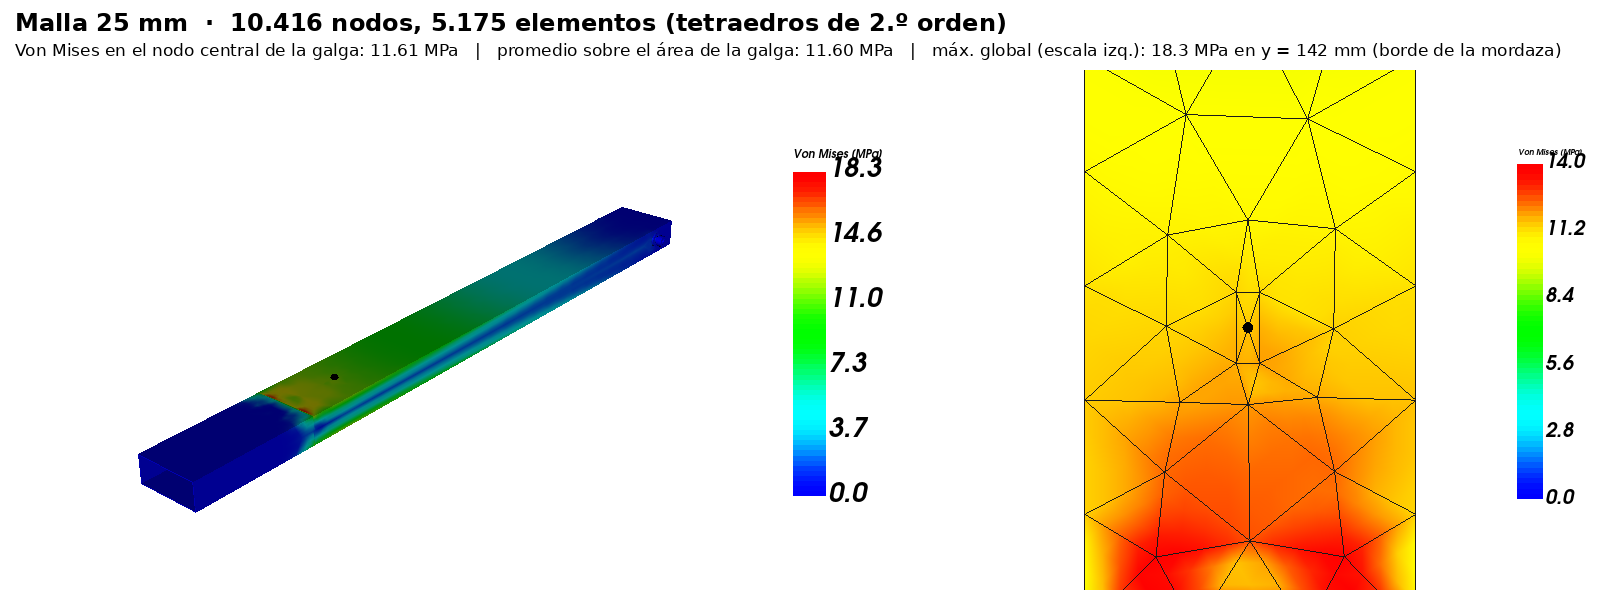
\includegraphics[width=\textwidth]{vm_25mm.png}
\caption{Malla de \SI{25}{mm}.}\label{fig:m25}
\end{figure}
\begin{figure}[H]\centering
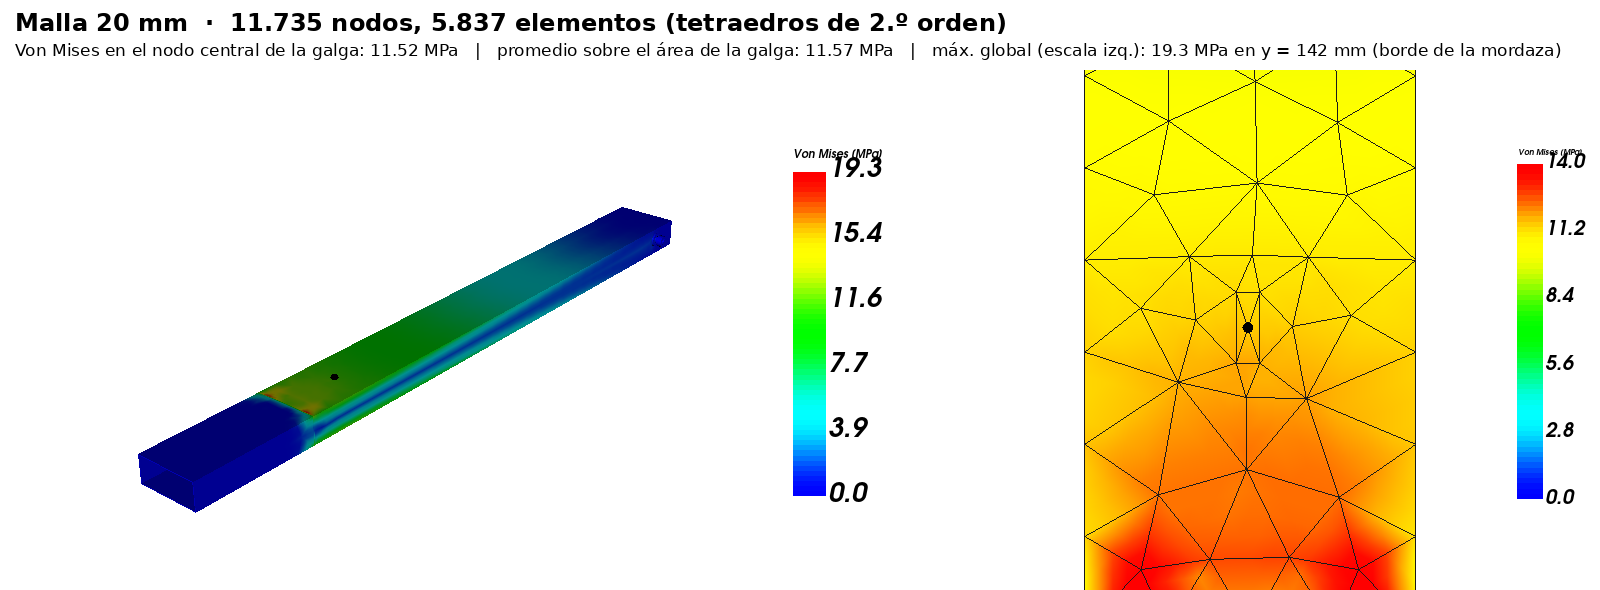
\includegraphics[width=\textwidth]{vm_20mm.png}
\caption{Malla de \SI{20}{mm}.}
\end{figure}
\begin{figure}[H]\centering
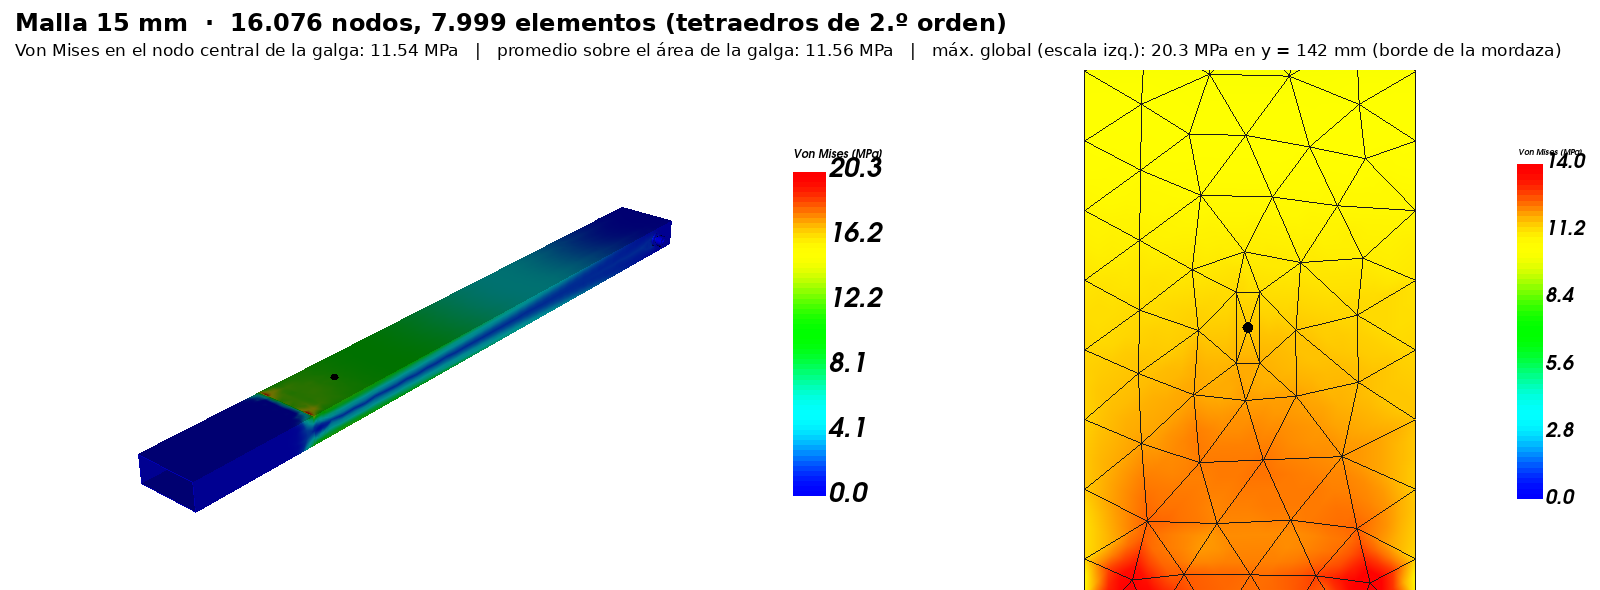
\includegraphics[width=\textwidth]{vm_15mm.png}
\caption{Malla de \SI{15}{mm}.}
\end{figure}
\begin{figure}[H]\centering
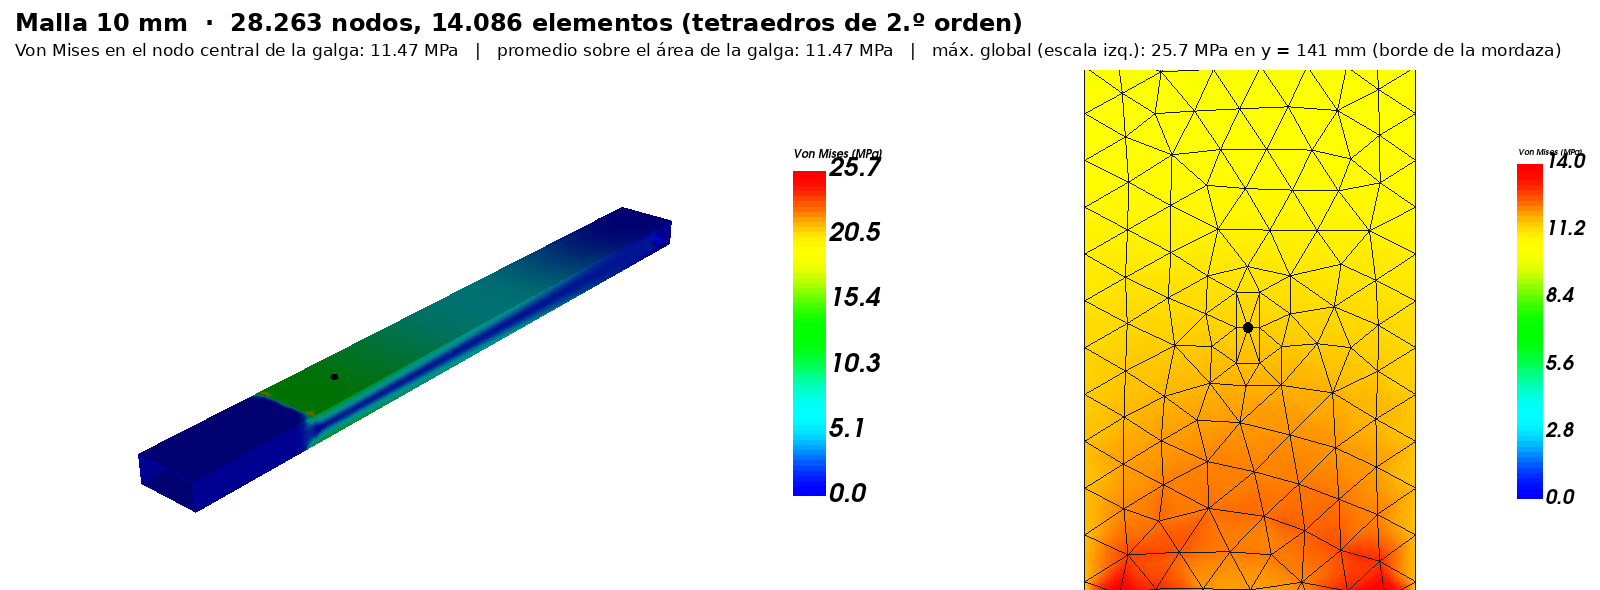
\includegraphics[width=\textwidth]{vm_10mm.png}
\caption{Malla de \SI{10}{mm}.}
\end{figure}
\begin{figure}[H]\centering
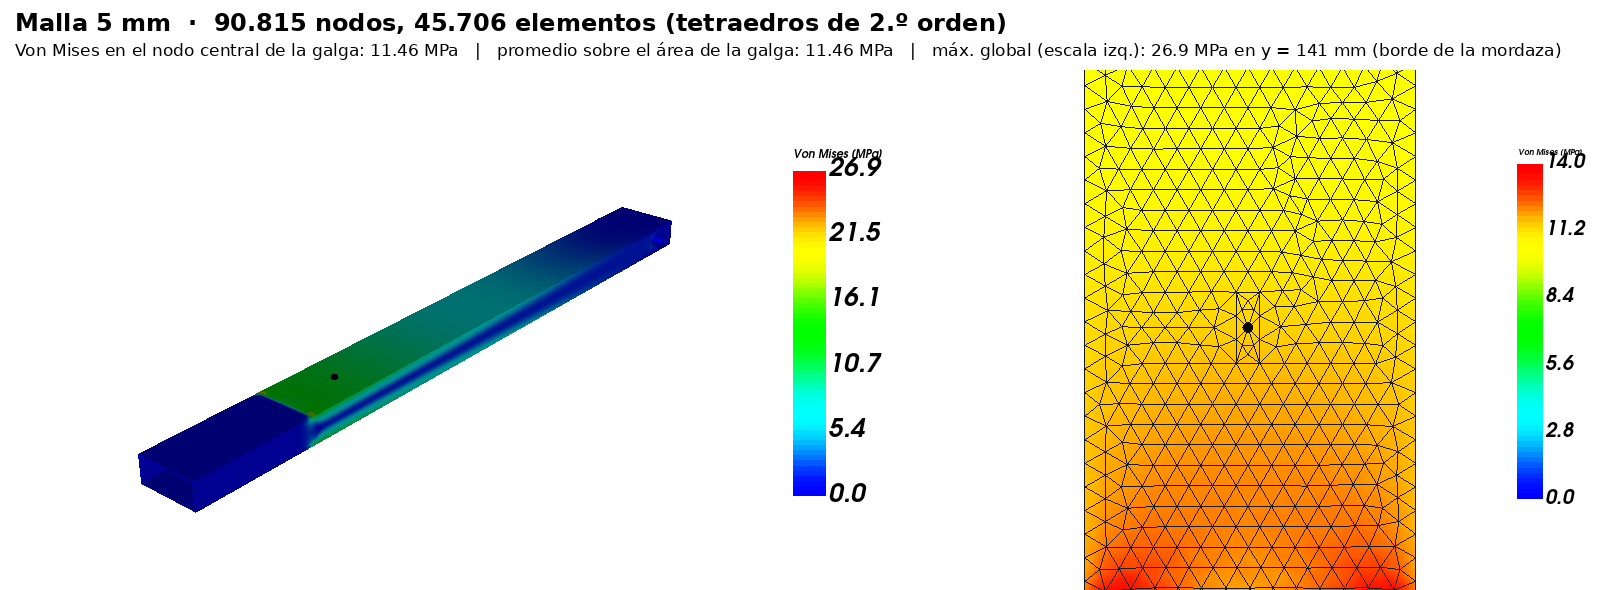
\includegraphics[width=\textwidth]{vm_5mm.png}
\caption{Malla de \SI{5}{mm}, usada como resultado. El punto negro marca el centro de la galga. Las im\'agenes se generaron por c\'odigo (VTK) a partir de los resultados de CalculiX, representando los elementos cuadr\'aticos de 10 nodos; las l\'ineas del acercamiento son las aristas de los elementos.}\label{fig:m5}
\end{figure}

\subsection{Esfuerzo de Von Mises en la galga}
El enunciado pide el esfuerzo de Von Mises en la galga; para comparar con la teor\'ia de vigas ($\sigma=Mc/I$) y con la galga se usan adem\'as el esfuerzo normal longitudinal $\sigma_{yy}$ y la deformaci\'on $\varepsilon_{yy}$. Cada magnitud se da en el nodo central de la galga y como promedio sobre su \'area. Con la malla de \SI{5}{mm}:
\begin{center}
\begin{tabular}{lrr}
\toprule
 & Nodo central & Promedio sobre el \'area \\
\midrule
\textbf{Von Mises} & \textbf{\SI{11,46}{MPa}} & \textbf{\SI{11,46}{MPa}} \\
$\sigma_{yy}$ & \SI{11,44}{MPa} & \SI{11,44}{MPa} \\
$\varepsilon_{yy}=[\sigma_{yy}-\nu(\sigma_{xx}+\sigma_{zz})]/E$ & \SI{166,04}{\microstrain} & \SI{166,04}{\microstrain} \\
\midrule
Diferencia de $\sigma_{yy}$ vs.\ anal\'itico (\SI{11,40}{MPa}) & \SI{+0,4}{\percent} & \SI{+0,4}{\percent} \\
Diferencia de Von Mises vs.\ anal\'itico & \SI{+0,6}{\percent} & \SI{+0,6}{\percent} \\
\bottomrule
\end{tabular}
\end{center}

\paragraph{Promedio sobre el \'area de la galga.} La galga no mide en un punto: mide la deformaci\'on promedio sobre su rejilla. Por eso, adem\'as del nodo central, se calcul\'o el promedio ponderado por \'area sobre la cara de la galga en el CAD ($5\times15$~mm, \SI{75}{mm^2}). Como la malla respeta el contorno de esa cara, se tomaron las caras de los elementos (tri\'angulos de 6 nodos) que la forman, se interpol\'o el tensor de esfuerzos con sus funciones de forma cuadr\'aticas y se integr\'o con una cuadratura de 6 puntos por tri\'angulo:
\begin{equation}
\bar{\sigma}=\frac{1}{A}\int_A \sigma\,dA\approx\frac{1}{A}\sum_{e}A_e\sum_{q=1}^{6}w_q\,\sigma(\xi_q),\qquad A=\sum_e A_e=\SI{75}{mm^2}.
\end{equation}
El \'area integrada es exactamente \SI{75}{mm^2} en todas las mallas, lo que confirma que se tom\'o la cara completa. El promedio y el valor central coinciden en menos del \SI{0,03}{\percent}, porque el momento flector var\'ia linealmente a lo largo de la galga y el promedio de una variaci\'on lineal es el valor en el centro; el promedio, sin embargo, depende menos de un nodo particular y es la magnitud m\'as cercana a lo que registra la galga. La rejilla sensible real puede ser m\'as peque\~na que la marca del CAD, pero al estar centrada el promedio no cambia por esa raz\'on.

\paragraph{Nodos que entran en el promedio.} Para que se vea de d\'onde sale el promedio y no solo el valor de un nodo, la figura~\ref{fig:nodos} muestra la cara de la galga en la malla de \SI{5}{mm}: contiene \num{49} nodos (\num{15} v\'ertices de los \num{20} tri\'angulos y \num{34} nodos intermedios de los elementos parab\'olicos), y la tabla~\ref{tab:nodos} da el esfuerzo en cada uno. El $\sigma_{yy}$ nodal va de \SI{11,25}{MPa} (en $y=\SI{213}{mm}$, el extremo m\'as alejado de la mordaza) a \SI{11,65}{MPa} (en $y=\SI{198}{mm}$) y baja de forma lineal con $y$, como el momento flector; en cada fila de $y$ los nodos de distinto $x$ dan el mismo valor (diferencias de pocas mil\'esimas de MPa), as\'i que no hay variaci\'on apreciable a lo ancho de la galga. La media aritm\'etica de los \num{49} nodos es \SI{11,445}{MPa} en $\sigma_{yy}$ y \SI{11,463}{MPa} en Von Mises, y coincide con el promedio ponderado por \'area (\SI{11,445}{MPa} y \SI{11,463}{MPa}); el nodo central (\SI{11,442}{MPa}) queda a \SI{0,03}{\percent} de ese promedio. Los nodos quedan unas cent\'esimas de MPa por encima de la recta de Mc/I (+\SI{0,4}{\percent}), la misma diferencia que se reporta en la tabla anterior.

\begin{figure}[H]
\centering
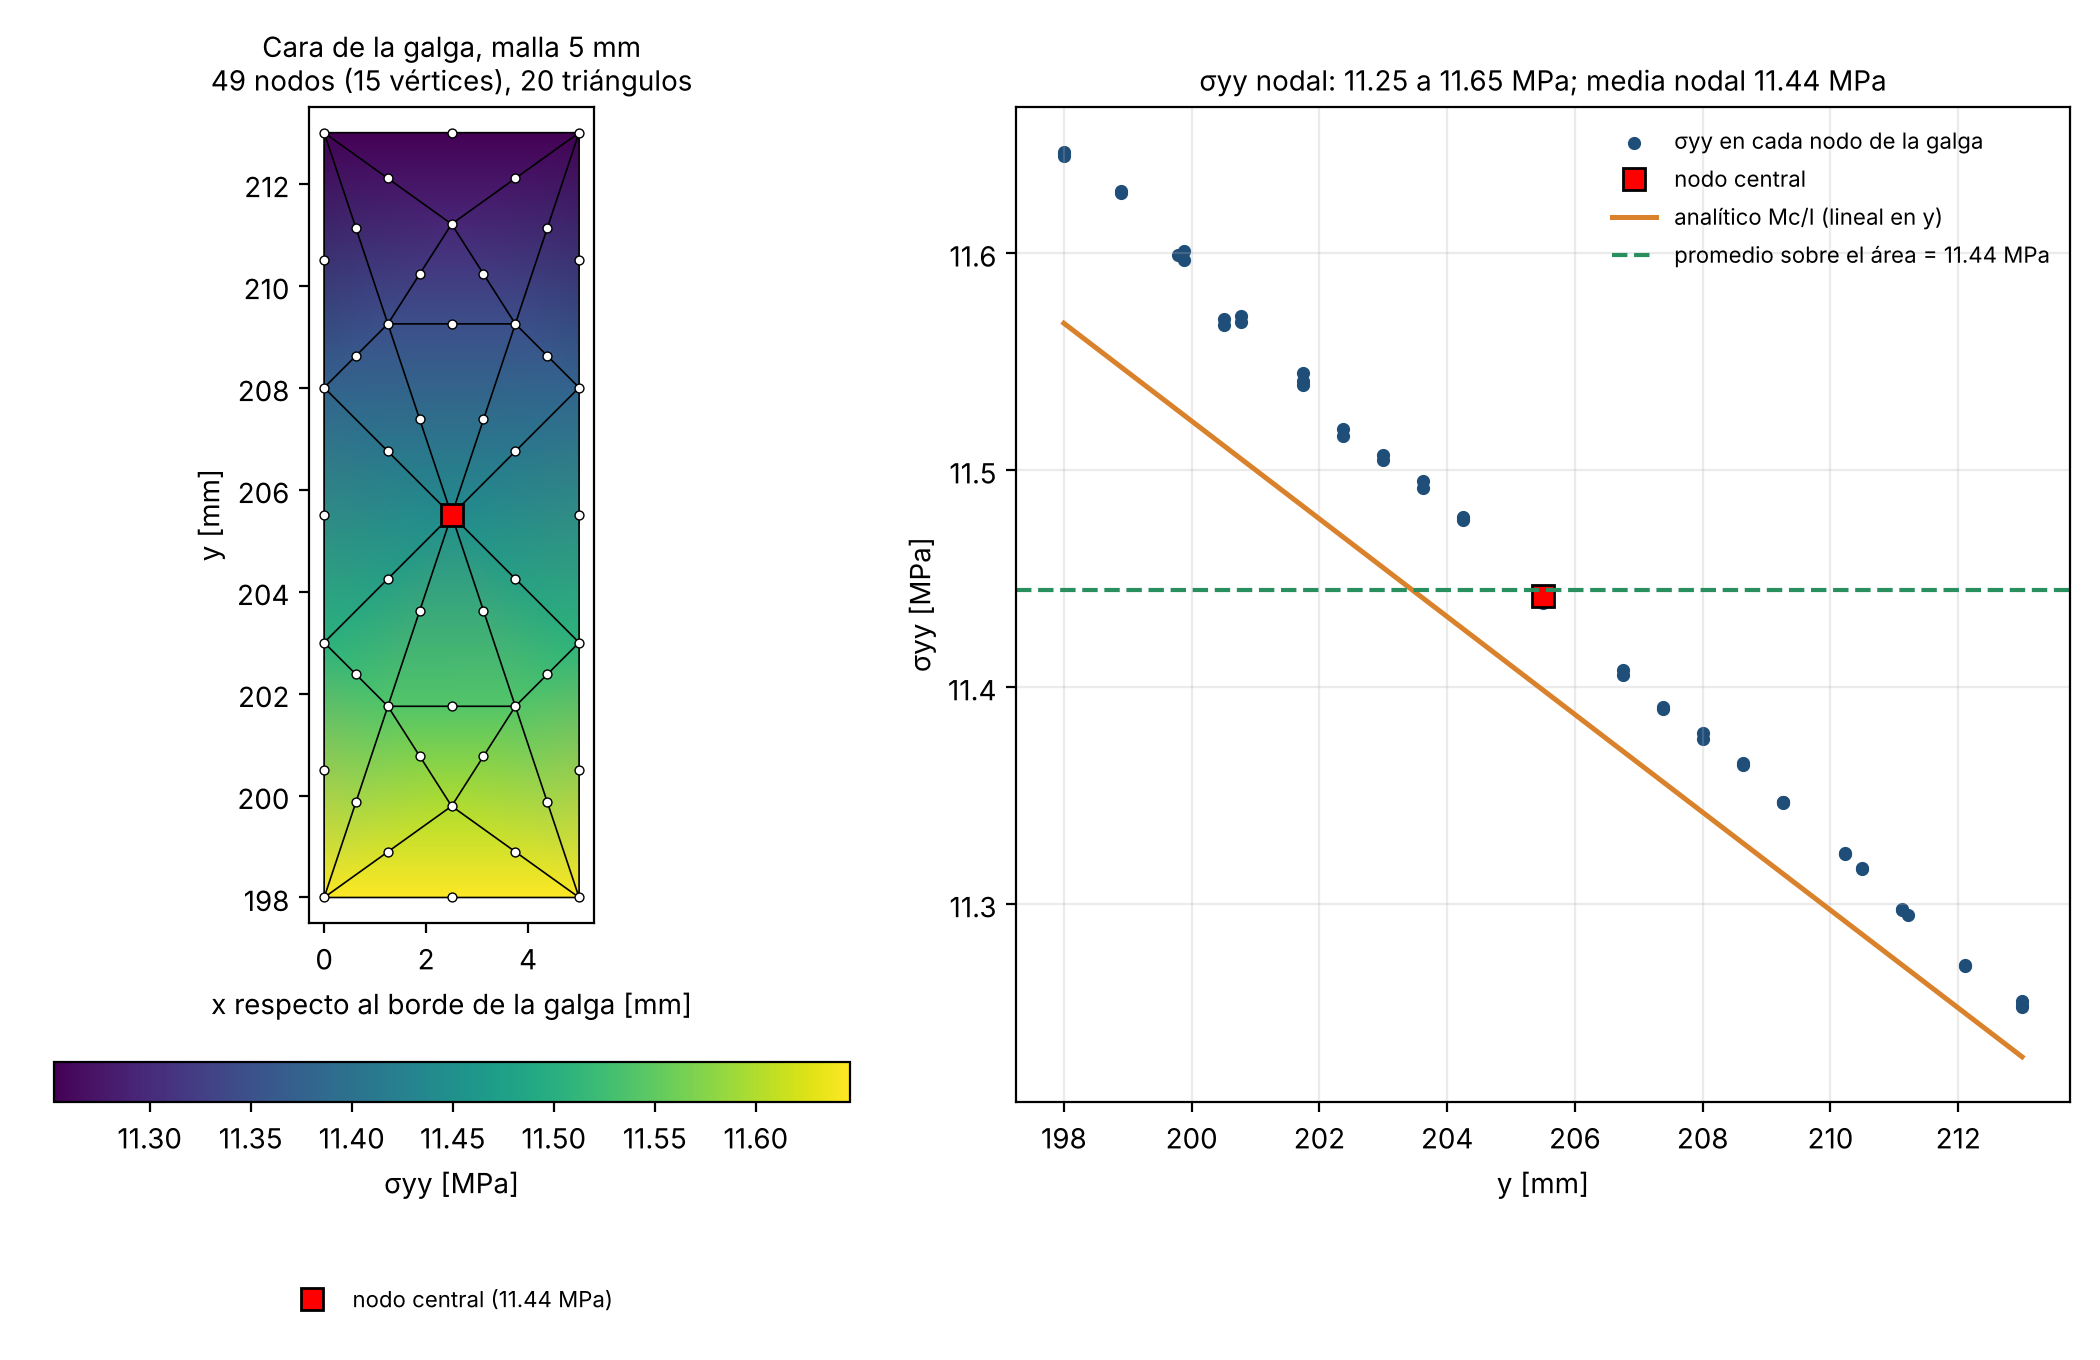
\includegraphics[width=\textwidth]{fig_nodos_galga_5mm.png}
\caption{Nodos de la cara de la galga (malla de \SI{5}{mm}). Izquierda: tri\'angulos y nodos sobre el parche de $5\times15$~mm, coloreados por $\sigma_{yy}$ (cuadrado rojo: nodo central). Derecha: $\sigma_{yy}$ de cada nodo contra $y$, la recta anal\'itica $Mc/I$ y el promedio sobre el \'area.}
\label{fig:nodos}
\end{figure}

{\footnotesize
\setlength{\tabcolsep}{4pt}
\begin{longtable}{rcrrrrrrr}
\caption{Esfuerzo en los nodos de la cara de la galga (malla de \SI{5}{mm}, \SI{49}{} nodos). V = v\'ertice, I = nodo intermedio; $x$ medido en el modelo CAD; tensiones en MPa; $\varepsilon_{yy}$ en \si{\microstrain}. Fila resaltada: nodo central.}\label{tab:nodos}\\
\toprule
Nodo & Tipo & $x$ [mm] & $y$ [mm] & $\sigma_{xx}$ & $\sigma_{yy}$ & $\sigma_{zz}$ & Von Mises & $\varepsilon_{yy}$ \\
\midrule
\endfirsthead
\toprule
Nodo & Tipo & $x$ [mm] & $y$ [mm] & $\sigma_{xx}$ & $\sigma_{yy}$ & $\sigma_{zz}$ & Von Mises & $\varepsilon_{yy}$ \\
\midrule
\endhead
\midrule \multicolumn{9}{r}{\emph{contin\'ua}}\\
\endfoot
\midrule
\multicolumn{5}{l}{Media aritm\'etica de los nodos} & \num{11,445} & & \num{11,463} & \\
\multicolumn{5}{l}{Promedio ponderado por \'area (\SI{75}{mm^2})} & \num{11,445} & & \num{11,463} & \num{166,04} \\
\bottomrule
\endlastfoot
37 & V & 14,07 & 198,00 & -0,001 & 11,646 & 0,005 & 11,645 & 168,76 \\
1278 & I & 16,57 & 198,00 & -0,004 & 11,645 & 0,006 & 11,644 & 168,76 \\
41 & V & 19,07 & 198,00 & 0,001 & 11,646 & 0,002 & 11,645 & 168,77 \\
14735 & I & 15,32 & 198,90 & -0,001 & 11,628 & 0,015 & 11,621 & 168,45 \\
14734 & I & 17,82 & 198,90 & 0,001 & 11,629 & 0,019 & 11,619 & 168,44 \\
14733 & V & 16,57 & 199,79 & -0,009 & 11,599 & 0,006 & 11,600 & 168,11 \\
1257 & I & 14,69 & 199,88 & -0,015 & 11,597 & 0,010 & 11,600 & 168,09 \\
1272 & I & 18,44 & 199,88 & -0,011 & 11,601 & 0,013 & 11,600 & 168,12 \\
1264 & I & 14,07 & 200,50 & -0,027 & 11,567 & -0,017 & 11,589 & 167,84 \\
1277 & I & 19,07 & 200,50 & -0,024 & 11,569 & -0,016 & 11,590 & 167,87 \\
14736 & I & 15,94 & 200,77 & -0,018 & 11,571 & -0,002 & 11,581 & 167,79 \\
14738 & I & 17,19 & 200,77 & -0,021 & 11,568 & -0,009 & 11,584 & 167,80 \\
1256 & V & 15,32 & 201,75 & -0,030 & 11,539 & -0,009 & 11,559 & 167,42 \\
14737 & I & 16,57 & 201,75 & -0,023 & 11,545 & 0,006 & 11,553 & 167,40 \\
1270 & V & 17,82 & 201,75 & -0,029 & 11,541 & -0,008 & 11,559 & 167,44 \\
14725 & I & 14,69 & 202,38 & -0,036 & 11,516 & -0,018 & 11,543 & 167,15 \\
14731 & I & 18,44 & 202,38 & -0,034 & 11,519 & -0,015 & 11,543 & 167,17 \\
1262 & V & 14,07 & 203,00 & -0,033 & 11,505 & -0,004 & 11,524 & 166,91 \\
1274 & V & 19,07 & 203,00 & -0,031 & 11,507 & -0,004 & 11,525 & 166,93 \\
1258 & I & 15,94 & 203,62 & -0,033 & 11,492 & -0,004 & 11,511 & 166,73 \\
1271 & I & 17,19 & 203,62 & -0,031 & 11,495 & -0,001 & 11,511 & 166,74 \\
14726 & I & 15,32 & 204,25 & -0,034 & 11,477 & 0,006 & 11,491 & 166,47 \\
14732 & I & 17,82 & 204,25 & -0,032 & 11,478 & 0,003 & 11,493 & 166,49 \\
1265 & I & 14,07 & 205,50 & -0,041 & 11,439 & -0,005 & 11,463 & 166,00 \\
\rowcolor{yellow!25} 38 & V & 16,57 & 205,50 & -0,040 & 11,442 & -0,004 & 11,464 & 166,04 \\
1276 & I & 19,07 & 205,50 & -0,040 & 11,441 & -0,006 & 11,464 & 166,03 \\
14728 & I & 15,32 & 206,75 & -0,047 & 11,405 & -0,009 & 11,434 & 165,57 \\
14729 & I & 17,82 & 206,75 & -0,044 & 11,408 & -0,008 & 11,434 & 165,58 \\
1261 & I & 15,94 & 207,38 & -0,050 & 11,390 & -0,004 & 11,417 & 165,33 \\
1268 & I & 17,19 & 207,38 & -0,048 & 11,391 & -0,004 & 11,417 & 165,33 \\
1263 & V & 14,07 & 208,00 & -0,044 & 11,376 & -0,002 & 11,400 & 165,09 \\
1273 & V & 19,07 & 208,00 & -0,043 & 11,379 & -0,002 & 11,401 & 165,12 \\
14727 & I & 14,69 & 208,62 & -0,044 & 11,364 & 0,007 & 11,383 & 164,88 \\
14730 & I & 18,44 & 208,62 & -0,044 & 11,365 & 0,004 & 11,385 & 164,90 \\
1259 & V & 15,32 & 209,25 & -0,048 & 11,347 & -0,000 & 11,371 & 164,68 \\
14880 & I & 16,57 & 209,25 & -0,049 & 11,346 & -0,004 & 11,373 & 164,69 \\
1267 & V & 17,82 & 209,25 & -0,047 & 11,347 & -0,002 & 11,372 & 164,69 \\
14883 & I & 15,94 & 210,23 & -0,050 & 11,323 & 0,001 & 11,348 & 164,33 \\
14884 & I & 17,19 & 210,23 & -0,049 & 11,323 & 0,001 & 11,348 & 164,34 \\
1266 & I & 14,07 & 210,50 & -0,045 & 11,316 & 0,001 & 11,339 & 164,21 \\
1275 & I & 19,07 & 210,50 & -0,046 & 11,316 & -0,000 & 11,340 & 164,22 \\
1260 & I & 14,69 & 211,12 & -0,050 & 11,297 & -0,005 & 11,326 & 164,00 \\
1269 & I & 18,44 & 211,12 & -0,050 & 11,298 & -0,005 & 11,326 & 164,00 \\
14879 & V & 16,57 & 211,21 & -0,054 & 11,295 & -0,001 & 11,322 & 163,95 \\
14881 & I & 15,32 & 212,10 & -0,054 & 11,271 & -0,002 & 11,299 & 163,62 \\
14882 & I & 17,82 & 212,10 & -0,053 & 11,272 & -0,002 & 11,299 & 163,62 \\
39 & V & 14,07 & 213,00 & -0,050 & 11,252 & -0,001 & 11,279 & 163,32 \\
1371 & I & 16,57 & 213,00 & -0,051 & 11,255 & 0,003 & 11,279 & 163,35 \\
40 & V & 19,07 & 213,00 & -0,050 & 11,254 & -0,001 & 11,279 & 163,33 \\
\end{longtable}
}

\paragraph{Estado de esfuerzo en la galga.} Que la galga est\'e en una cara libre no garantiza por s\'i solo un estado uniaxial; lo que lo respalda es el tensor completo calculado en el centro de la galga (malla de \SI{5}{mm}):
\begin{center}
\small
\begin{tabular}{cccccc}
\toprule
$\sigma_{xx}$ & $\sigma_{yy}$ & $\sigma_{zz}$ & $\tau_{xy}$ & $\tau_{yz}$ & $\tau_{zx}$ \\
\midrule
$-0{,}040$ & $11{,}442$ & $-0{,}004$ & $-0{,}012$ & $-0{,}001$ & $0{,}000$ \\
\bottomrule
\end{tabular}

\smallskip
Componentes en MPa.
\end{center}
Todas las componentes distintas de $\sigma_{yy}$ son menores que el \SI{0,4}{\percent} de este, de modo que la aproximaci\'on uniaxial $\sigma=E\varepsilon$ usada en la Parte~2 es adecuada aqu\'i. La deformaci\'on longitudinal con el tensor completo es $\varepsilon_{yy}=\SI{166,04}{\microstrain}$, solo \SI{0,13}{\percent} mayor que $\sigma_{yy}/E=\SI{165,82}{\microstrain}$; para comparar con la galga es preferible usar $\varepsilon_{yy}$.



\subsubsection{Verificaci\'on del modelo}
\begin{itemize}
\item \textbf{Equilibrio.} La suma de las reacciones en el apoyo es $R_z=\SI{49,766}{N}$ (y $R_x\approx R_y\approx0$), igual a la carga aplicada.
\item \textbf{Estudio de malla.} Ver la secci\'on anterior.
\item \textbf{Sensibilidad al apoyo.} Si en vez de las caras de la mordaza se empotra \'unicamente la cara del extremo ($y=0$), el resultado en la galga cambia $\SI{-0,60}{\percent}$ en Von Mises y $\SI{-0,41}{\percent}$ en $\sigma_{yy}$ (ambos \SI{11,39}{MPa}). La conclusi\'on se limita a esas dos idealizaciones del apoyo.
\item \textbf{Coherencia con la teor\'ia.} Seg\'un la teor\'ia de flexi\'on de vigas \cite{beer}, el esfuerzo en la fibra superior es $Mc/I$. El $\sigma_{yy}$ del FEM y la teor\'ia difieren \SI{0,4}{\percent}: los dos modelos son coherentes para la geometr\'ia y la carga nominales.
\end{itemize}

\paragraph{Limitaciones del modelo.}
\begin{itemize}
\item Las piezas est\'an pegadas entre s\'i (sin holgura ni fricci\'on en el agujero del tornillo), y las cuerdas se representan como dos fuerzas repartidas en el eje del tornillo mediante un acople r\'igido. Es una idealizaci\'on del montaje real.
\item En el espesor de \SI{1}{mm} la malla tiene un solo elemento parab\'olico (tres nodos, a $z=29$, $29{,}5$ y \SI{30}{mm}) en todos los tama\~nos probados, de modo que el tama\~no global cambia sobre todo la discretizaci\'on en el plano de la pared. El resultado coincide con la teor\'ia porque en flexi\'on global el esfuerzo es casi uniforme a trav\'es de una pared delgada, pero una comprobaci\'on adicional con m\'as elementos en el espesor reforzar\'ia la conclusi\'on.
\item El valor de Von Mises en un nodo proviene de la extrapolaci\'on de los puntos de integraci\'on del elemento, por lo que peque\~nas diferencias entre mallas (centésimas de MPa) est\'an dentro de lo esperable.
\end{itemize}

\paragraph{Alcance.} El FEM usa la geometr\'ia nominal (espesor \SI{1}{mm}, $E=\SI{69}{GPa}$) y est\'a de acuerdo con la teor\'ia. Esa coincidencia respalda la consistencia de ambos c\'alculos con las mismas entradas nominales, pero no identifica la causa de la diferencia con el ensayo (\SI{+10}{} a \SI{+12}{\percent}), que se analiza en la Parte~4.

\section{Parte 4: comparaci\'on de resultados y an\'alisis de errores}
\begin{quote}\small\textit{Resumen de la parte.} Se compara el esfuerzo normal longitudinal $\sigma_{yy}$ en la galga obtenido por el modelo anal\'itico, por el FEM y por el ensayo, para la carga de \SI{49,77}{N} (pesa m\'as herraje, ya que la galga se puso en cero antes de colgarlos). Tomando el valor anal\'itico como referencia, el $\sigma_{yy}$ del FEM difiere \SI{+0,4}{\percent} (el Von Mises que pide la Parte~3, \SI{+0,6}{\percent}) y el ensayo \SI{+10,1}{\percent}. Los modelos anal\'itico y FEM son coherentes para la geometr\'ia y la carga nominales. La diferencia con el ensayo puede relacionarse con las dimensiones reales de la viga, con la instrumentaci\'on y con simplificaciones del montaje; se analizan esos factores como sensibilidades, sin que los datos disponibles permitan determinar una causa \'unica.\end{quote}

\subsection{Resultados a comparar}
Para comparar la misma magnitud, los resultados corresponden al esfuerzo normal longitudinal $\sigma_{yy}$ en la galga (cara superior, centro en $y=\SI{205,5}{mm}$), para la carga de $P=\SI{49,77}{N}$: la galga se puso en cero antes de colgar el tornillo y las arandelas, as\'i que registra la pesa m\'as el herraje (confirmado por el profesor). Del FEM se dan dos lecturas: el valor en el nodo central y el promedio sobre el \'area de la galga (\SI{75}{mm^2}), que es lo m\'as parecido a lo que mide la galga (Parte~3).

\begin{table}[H]
\centering
\caption{Esfuerzo en la galga por cada m\'etodo.}
\begin{tabular}{lrl}
\toprule
M\'etodo & $\sigma$ [MPa] & Origen \\
\midrule
Anal\'itico, $Mc/I$ & 11,40 & Parte~1 \\
FEM, $\sigma_{yy}$ en el nodo central & 11,44 & Parte~3 (malla \SI{5}{mm}) \\
FEM, $\sigma_{yy}$ promedio sobre el \'area de la galga & 11,44 & Parte~3 (malla \SI{5}{mm}) \\
Ensayo, $E\varepsilon$ (l\'inea base restada) & 12,55 & Parte~2 \\
\midrule
FEM, Von Mises (nodo central / promedio \'area) & 11,46 / 11,46 & Parte~3 \\
\bottomrule
\end{tabular}
\end{table}
El Von Mises es el valor que pide la Parte~3, pero no es la misma magnitud que $Mc/I$; por eso la comparaci\'on se hace con $\sigma_{yy}$.

\subsection{Porcentajes de error respecto al resultado anal\'itico}
El error se calcula como
\begin{equation}
e\,[\%]=\frac{\sigma_\text{m\'etodo}-\sigma_\text{anal\'itico}}{\sigma_\text{anal\'itico}}\times100 .
\end{equation}

\begin{table}[H]
\centering
\caption{Error respecto al valor anal\'itico (\SI{11,40}{MPa}).}
\label{tab:err}
\begin{tabular}{lr}
\toprule
 & Error \\
\midrule
\textbf{FEM, $\sigma_{yy}$ en el nodo central} & \textbf{\SI{+0,38}{\percent}} \\
\textbf{FEM, $\sigma_{yy}$ promedio sobre el \'area de la galga} & \textbf{\SI{+0,40}{\percent}} \\
\textbf{Ensayo (con l\'inea base restada)} & \textbf{\SI{+10,1}{\percent}} \\
Ensayo sin restar la l\'inea base & \SI{+12,2}{\percent} \\
\midrule
Ensayo respecto al $\sigma_{yy}$ promedio del FEM & \SI{+9,6}{\percent} \\
Deformaci\'on del ensayo respecto a $\varepsilon_{yy}$ promedio del FEM (\SI{166,04}{\microstrain}) & \SI{+9,5}{\percent} \\
FEM, Von Mises (nodo central / promedio \'area, informativo) & \SI{+0,58}{\percent} / \SI{+0,57}{\percent} \\
\bottomrule
\end{tabular}
\end{table}

\begin{figure}[H]
\centering
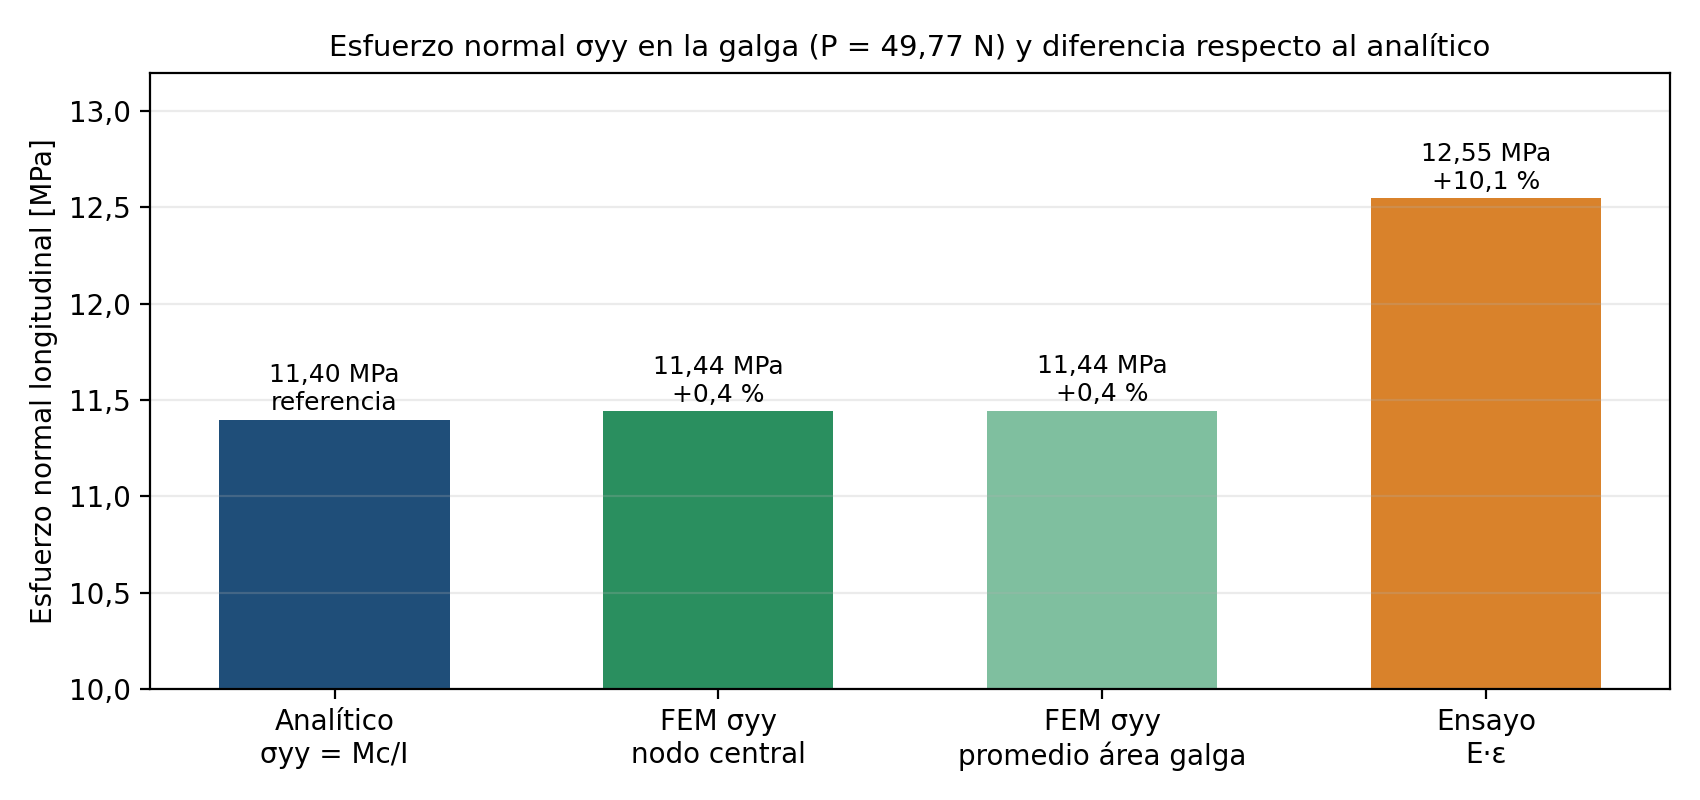
\includegraphics[width=0.85\textwidth]{fig_comparacion.png}
\caption{Esfuerzo normal $\sigma_{yy}$ en la galga por m\'etodo y diferencia respecto al valor anal\'itico.}
\end{figure}

El FEM queda a menos de medio punto porcentual del valor anal\'itico, tanto en el nodo central como en promedio sobre el \'area de la galga, y el ensayo un \SI{10}{\percent} por encima de ambos.

\subsection{An\'alisis de las causas de las diferencias}
\subsubsection{\texorpdfstring{FEM frente al anal\'itico (\SI{+0,4}{\percent})}{FEM frente al analitico (+0,4 \%)}}
Es una diferencia peque\~na y esperable entre un modelo tridimensional y la teor\'ia de vigas \cite{beer}:
\begin{itemize}
\item El modelo 3D incluye la zona del apoyo, el agujero del tornillo y las uniones entre piezas, que la teor\'ia de vigas no considera. La galga est\'a a \SI{64}{mm} del borde de la mordaza, lo bastante lejos para que su efecto local sea peque\~no.
\item La variaci\'on del resultado entre las mallas comparadas (10 a \SI{4}{mm}) es menor que \SI{0,1}{\percent} (Parte~3).
\item La forma de modelar el apoyo cambia $\sigma_{yy}$ en $\SI{-0,41}{\percent}$ (Parte~3), del mismo orden que la diferencia observada.
\end{itemize}
Como el FEM usa la misma geometr\'ia y el mismo material que la teor\'ia, esta coincidencia respalda la consistencia de los dos c\'alculos para las mismas entradas nominales. Pero ambos pueden compartir hip\'otesis que no reflejen el montaje real, as\'i que la coincidencia \textbf{no identifica la causa} de la diferencia con el ensayo.

\subsubsection{\texorpdfstring{Ensayo frente al anal\'itico (\SI{+10,1}{\percent})}{Ensayo frente al analitico (+10,1 \%)}}
Como la teor\'ia y el FEM coinciden para las entradas nominales, la diferencia puede relacionarse con que el montaje real difiere del modelo nominal, con la medici\'on o con hip\'otesis compartidas por ambos modelos. La tabla~\ref{tab:causas} resume los factores considerados y la figura~\ref{fig:sens} muestra cu\'anto cambiar\'ia el valor te\'orico con cambios de ejemplo en cada par\'ametro. Son an\'alisis de sensibilidad: los tama\~nos de los cambios son ilustrativos, no incertidumbres medidas.

Los factores se agrupan en cinco categor\'ias: la galga y su instrumentaci\'on, las condiciones f\'isicas de la viga, los procedimientos del ensayo y las simplificaciones del modelo anal\'itico y del FEM. La columna ``efecto'' dice cu\'anto cambiar\'ia el resultado y en qu\'e sentido; los factores no cuantificados se se\~nalan como tales.

{\small
\begin{longtable}{p{3.4cm}p{6.9cm}p{4.2cm}}
\caption{Fuentes de diferencia entre el ensayo y los modelos, por categor\'ia.}\label{tab:causas}\\
\toprule
Fuente & Efecto (magnitud y sentido) & Referencia / estado \\
\midrule
\endfirsthead
\toprule
Fuente & Efecto (magnitud y sentido) & Referencia / estado \\
\midrule
\endhead
\multicolumn{3}{l}{\textbf{A. Galga e instrumentaci\'on}}\\
\addlinespace
Factor de galga mal ingresado & El error en la deformaci\'on mostrada es uno a uno con el error del factor: un desajuste de \SI{3}{\percent} mueve el resultado \SI{3}{\percent}; de \SI{5}{\percent}, la diferencia baja a $\approx\SI{+4,6}{\percent}$ (Parte~2). Con todo lo dem\'as fijo, un cociente $GF_\text{conf}/GF_\text{real}=0{,}908$ igualar\'ia num\'ericamente ensayo y teor\'ia. & \cite{watson}. Seg\'un el profesor, su efecto es peque\~no; no se cuantific\'o. \\
\addlinespace
Sensibilidad transversal & Con $K_t\approx\SI{1}{\percent}$ y esfuerzo uniaxial en aluminio ($\nu=0{,}33$ frente a \num{0,285} de calibraci\'on), el error es del orden de \SI{0,05}{\percent}: despreciable. & \cite{tn509}; c\'alculo propio. \\
\addlinespace
Desalineaci\'on de la galga & Con \SI{5}{^\circ} de desalineaci\'on la lectura baja $\approx\SI{1}{\percent}$. Reduce la lectura, as\'i que aumentar\'ia la diferencia; no la explica. & \cite{tn511}; c\'alculo propio. \\
\addlinespace
Cables y puente & La atenuaci\'on por la resistencia de los cables es un error com\'un y baja la lectura. No cuantificado (depende de la longitud y del tipo de puente). & \cite{hernik}. Configuraci\'on no disponible. \\
\addlinespace
Temperatura y deriva del cero & Restar la l\'inea base corrige el desplazamiento de referencia; la deriva residual durante la meseta no est\'a cuantificada. & \cite{tn504}. \\
\addlinespace
Excitaci\'on, adhesi\'on e instalaci\'on & Una excitaci\'on excesiva o un pegado defectuoso causan deriva o transmisi\'on incompleta de la deformaci\'on. No cuantificado; la se\~nal estable en la meseta no muestra deriva apreciable. & \cite{watson}. \\
\midrule
\multicolumn{3}{l}{\textbf{B. Condiciones f\'isicas de la viga y de la carga}}\\
\addlinespace
\textbf{Espesor de pared} & Espesor \SI{0,95}{mm}: el valor te\'orico sube \SI{4,8}{\percent}; \SI{0,90}{mm}: sube \SI{10,2}{\percent}. Con todo lo dem\'as fijo, \SI{0,901}{mm} igualar\'ia num\'ericamente teor\'ia y ensayo (sensibilidad matem\'atica, no evidencia). Es el par\'ametro geom\'etrico de mayor efecto porque $I$ depende de $t$. & No medido; se usa el nominal. \\
\addlinespace
Altura y ancho de la secci\'on & Altura \SI{29,5}{mm} en lugar de \SI{30}{mm}: $\SI{+2,0}{\percent}$. & No medidos. \\
\addlinespace
Posici\'on de la galga & Galga \SI{10}{mm} m\'as cerca de la mordaza: $\SI{+2,0}{\percent}$. & Tomada del CAD. \\
\addlinespace
Brazo de carga & Punto de carga \SI{5}{mm} m\'as lejos: $\SI{+1,0}{\percent}$. & Tomado del CAD. \\
\addlinespace
Masa colgada & $\pm\SI{1}{\percent}$ de masa: $\SI{\pm1,0}{\percent}$. & No verificada con balanza. \\
\addlinespace
M\'odulo de elasticidad & Un $E$ real \SI{3}{\percent} menor aumentar\'ia la deformaci\'on esperada \SI{3}{\percent}; para el aluminio 1100 las variaciones esperables son menores. & \cite{asm}. Efecto peque\~no. \\
\addlinespace
Rigidez del apoyo & La viga en voladizo es isost\'atica: el momento en la galga no depende de la rigidez de la mordaza. En el FEM, cambiar el apoyo modifica $\sigma_{yy}$ en $\SI{-0,41}{\percent}$ (Von Mises, $\SI{-0,60}{\percent}$). & Parte~3. \\
\midrule
\multicolumn{3}{l}{\textbf{C. Procedimientos del ensayo}}\\
\addlinespace
Estado del cero (herraje) & El profesor confirm\'o que el cero se tom\'o sin el herraje: la carga de comparaci\'on es \SI{49,77}{N}. Si se hubiera tomado con el herraje, la diferencia subir\'ia \SI{1,6}{} puntos. & Confirmado. \\
\addlinespace
L\'inea base y ventana de promedio & Restar la l\'inea base baja el resultado $\approx\SI{2}{}$ puntos (\SI{12,2}{} a \SI{10,1}{\percent}); cambiar la ventana de la meseta casi no lo afecta ($<\SI{0,03}{\microstrain}$). & Parte~2. \\
\addlinespace
Medidas manuales (distancias, masa) & Cada \SI{5}{mm} de error en un brazo vale $\approx\SI{1}{\percent}$ (ver arriba). & Procedimiento de laboratorio. \\
\midrule
\multicolumn{3}{l}{\textbf{D. Simplificaciones del modelo anal\'itico}}\\
\addlinespace
Teor\'ia de Euler--Bernoulli & Desprecia la deformaci\'on por cortante y los efectos locales. El FEM 3D, que s\'i los incluye, difiere solo \SI{0,4}{\percent} en $\sigma_{yy}$: el efecto es peque\~no en la posici\'on de la galga. & \cite{beer}. \\
\addlinespace
Geometr\'ia nominal & Se usa secci\'on rectangular con esquinas vivas y espesor uniforme. Los radios de esquina y las tolerancias de los perfiles comerciales cambian $I$; no cuantificado. & No medidos. \\
\addlinespace
Peso propio excluido & Aportar\'ia $\approx\SI{0,34}{MPa}$ ($\approx\SI{3}{\percent}$), pero la galga se puso en cero con la viga montada. & Parte~1. \\
\midrule
\multicolumn{3}{l}{\textbf{E. Simplificaciones del FEM}}\\
\addlinespace
Discretizaci\'on & Variaci\'on menor que \SI{0,1}{\percent} entre las mallas de 10 a \SI{4}{mm} (no es una cota demostrada del error). Hay un solo elemento parab\'olico en el espesor de \SI{1}{mm} en todas las mallas. & Parte~3. \\
\addlinespace
Uniones pegadas y acople r\'igido & El tornillo y las cuerdas se idealizan; la zona de carga est\'a a $\approx\SI{500}{mm}$ de la galga, por lo que su efecto all\'i es peque\~no (principio de Saint-Venant). & \cite{beer}. No cuantificado. \\
\addlinespace
Material lineal con valores nominales & Con $E$ y $\nu$ nominales; en una viga isost\'atica, el esfuerzo casi no depende de $E$. & \cite{asm}. \\
\addlinespace
Lectura nodal de Von Mises & Valor extrapolado de los puntos de integraci\'on; variaciones de cent\'esimas de MPa entre mallas. Von Mises y $\sigma_{yy}$ difieren \SI{0,02}{MPa}, y el promedio sobre el \'area de la galga coincide con el nodo central en menos del \SI{0,03}{\percent}. & Parte~3. \\
\bottomrule
\end{longtable}
}

\begin{figure}[H]
\centering
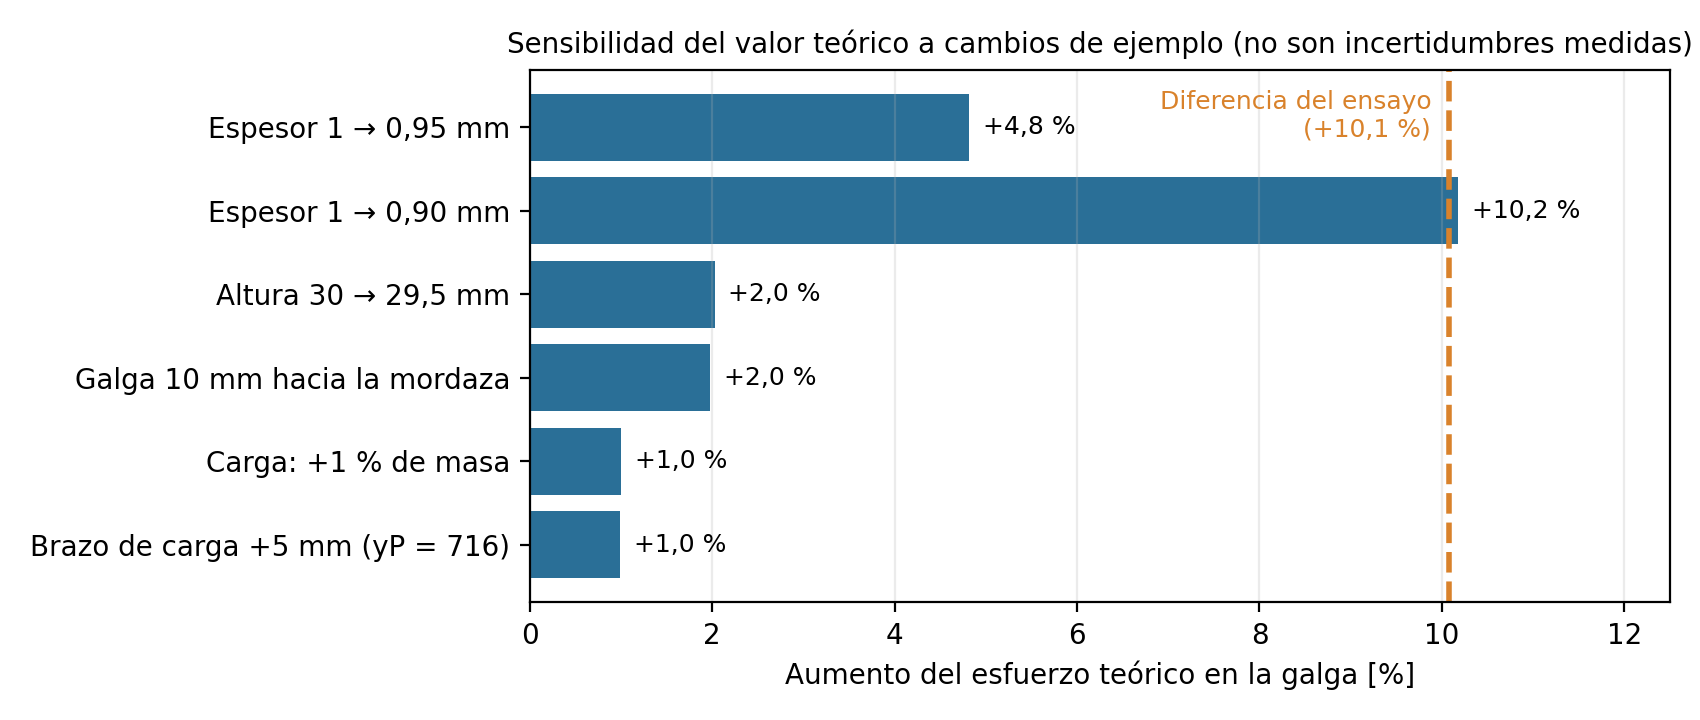
\includegraphics[width=0.85\textwidth]{fig_sensibilidad.png}
\caption{Aumento del esfuerzo te\'orico en la galga ante cambios de ejemplo de cada par\'ametro, comparado con la diferencia del ensayo (\SI{+10,1}{\percent}).}
\label{fig:sens}
\end{figure}

\paragraph{Factores descartados o poco probables.}
\begin{itemize}
\item \textbf{Peso propio de la viga.} Aportar\'ia $\approx\SI{0,34}{MPa}$ ($\approx\SI{3}{\percent}$), pero la galga se puso en cero con la viga montada, de modo que ya est\'a descontado.
\item \textbf{Efectos din\'amicos.} La se\~nal en la meseta es estable (desviaci\'on est\'andar \SI{0,86}{\microstrain}, sin tendencia apreciable), as\'i que la medici\'on corresponde a una carga est\'atica.
\item \textbf{Estado no uniaxial.} El tensor de esfuerzos del FEM en la galga tiene componentes distintas de $\sigma_{yy}$ menores que el \SI{0,4}{\percent} de este (Parte~3); usar $\varepsilon_{yy}$ del FEM en vez de $\sigma_{yy}/E$ cambia la comparaci\'on solo \SI{0,13}{\percent}.
\item \textbf{Orientaci\'on de la galga.} Una galga desalineada del eje $y$ mide menos deformaci\'on longitudinal, no m\'as: no explica una lectura alta.
\end{itemize}

\subsubsection{Verificaci\'on y validaci\'on}
La literatura de simulaci\'on distingue dos preguntas \cite{asme,oberkampf}. La \emph{verificaci\'on} comprueba que el modelo resuelve correctamente las ecuaciones que se le plantean: aqu\'i, el estudio de malla (Parte~3), el equilibrio de reacciones y la coincidencia con la soluci\'on anal\'itica ($\SI{+0,4}{\percent}$ en $\sigma_{yy}$). La \emph{validaci\'on} comprueba que el modelo representa la realidad: aqu\'i, la comparaci\'on con el ensayo ($\SI{+10,1}{\percent}$). Una verificaci\'on satisfactoria indica que el solver resuelve bien el modelo planteado; la diferencia de validaci\'on puede deberse a las entradas del modelo (geometr\'ia, carga, posiciones), a hip\'otesis compartidas por la teor\'ia y el FEM, o a la medici\'on. Para cuantificarla con rigor, cada entrada debe medirse con su incertidumbre y propagarse al resultado seg\'un la gu\'ia GUM \cite{gum}; con los datos actuales solo se puede hacer an\'alisis de sensibilidad, como en esta secci\'on.

\subsubsection{Un escenario ilustrativo}
Con todo lo dem\'as fijo, un espesor de \SI{0,901}{mm} o un cociente de factores de galga de \num{0,908} igualar\'ian num\'ericamente teor\'ia y ensayo; son sensibilidades matem\'aticas, no evidencia de que haya ocurrido. La diferencia tambi\'en podr\'ia ser la suma de varios efectos peque\~nos. Como ilustraci\'on (no como medici\'on): con espesor de \SI{0,95}{mm}, galga \SI{5}{mm} m\'as cerca de la mordaza y un factor de galga configurado \SI{3}{\percent} menor que el real, el valor te\'orico ser\'ia \SI{12,07}{MPa} y el medido corregido \SI{12,17}{MPa}, es decir, la diferencia bajar\'ia a $\SI{+0,9}{\percent}$. El escenario muestra que la magnitud de la diferencia es compatible con tolerancias de fabricaci\'on y de instrumentaci\'on, pero demostrarlo requiere medir esos par\'ametros.

\subsection{Conclusiones}
\begin{enumerate}
\item El esfuerzo normal $\sigma_{yy}$ del FEM difiere \SI{+0,4}{\percent} del valor anal\'itico, tanto en el nodo central como en promedio sobre el \'area de la galga (el Von Mises, \SI{+0,6}{\percent}). Los modelos anal\'itico y FEM son coherentes para la geometr\'ia y la carga nominales.
\item El ensayo da un esfuerzo equivalente $E\varepsilon$ \SI{10,1}{\percent} mayor que el anal\'itico (\SI{12,2}{\percent} si no se resta la l\'inea base), para la carga de \SI{49,77}{N} confirmada por el profesor.
\item La diferencia con el ensayo puede relacionarse con dimensiones reales, adquisici\'on y simplificaciones del montaje. Los datos disponibles no permiten determinar una causa \'unica ni cerrar la validaci\'on experimental.
\item Los factores se agrupan en galga, condiciones f\'isicas, procedimientos y simplificaciones del an\'alisis y del FEM (tabla~\ref{tab:causas}). Varios de ellos (espesor, factor de galga) podr\'ian por s\'i solos igualar num\'ericamente los resultados si sus valores reales fueran los adecuados, pero ninguno se ha medido.
\item Para cerrar la comparaci\'on con evidencia ser\'ia necesario medir el espesor y la altura de la secci\'on en varios puntos y la posici\'on real de la galga y del punto de carga, conocer la configuraci\'on de la galga en la adquisici\'on y evaluar la incertidumbre total del ensayo.
\end{enumerate}

\section{Conclusiones generales}
\begin{enumerate}
\item La soluci\'on anal\'itica (teor\'ia de vigas de Euler--Bernoulli) da $\sigma_{yy}=\SI{11,40}{MPa}$ (\SI{165,2}{\microstrain}) en la galga para una carga de \SI{49,77}{N}.
\item El FEM, con estudio de malla (variaci\'on menor que \SI{0,1}{\percent} entre las mallas de 10 a \SI{4}{mm}) y equilibrio de reacciones verificado, da en la galga un esfuerzo de Von Mises de \SI{11,46}{MPa} y $\sigma_{yy}=\SI{11,44}{MPa}$, iguales en el nodo central y en promedio sobre el \'area de la galga: \SI{+0,4}{\percent} respecto a la teor\'ia. El estado de esfuerzo en la galga es pr\'acticamente uniaxial.
\item El ensayo da \SI{181,85}{\microstrain} netos y $E\varepsilon=\SI{12,55}{MPa}$, es decir, \SI{+10,1}{\percent} respecto a la teor\'ia (\SI{+12,2}{\percent} sin restar la l\'inea base).
\item Los modelos anal\'itico y FEM son coherentes para la geometr\'ia y la carga nominales. La diferencia con el ensayo puede relacionarse con las dimensiones reales de la viga (en especial el espesor de pared), con la instrumentaci\'on (factor de galga, cables, deriva) y con simplificaciones del montaje; los datos disponibles no permiten determinar una causa \'unica.
\item Para cerrar la validaci\'on ser\'ia necesario medir el espesor y las dimensiones de la secci\'on y las posiciones reales de la galga y de la carga, conocer la configuraci\'on de la galga en la adquisici\'on y evaluar la incertidumbre total del ensayo.
\end{enumerate}

\section{Anexos}
\begin{itemize}
\item \textbf{Datos del ensayo:} \texttt{Viga4SamuelBrayan.csv} y resultados del procesamiento (\texttt{resultados\_exp.json}).
\item \textbf{CAD:} \texttt{VIGA\_FEM.step} (formato neutro) y archivo nativo de Autodesk Fusion.
\item \textbf{FEM:} archivos de entrada de CalculiX (\texttt{.inp}) y resultados (\texttt{.frd}) de las mallas de 25, 20, 15, 10, 7, 5 y \SI{4}{mm} y de la variante de apoyo en el extremo, extracci\'on de resultados en la galga (\texttt{galga\_fem.json}), valores nodales de la cara de la galga (\texttt{nodos\_galga\_5mm.csv}), scripts de mallado, c\'alculo y capturas.
\item \textbf{C\'odigo:} scripts de Python del an\'alisis anal\'itico, del tratamiento del ensayo y de la comparaci\'on.
\end{itemize}

\begin{thebibliography}{99}
\bibitem{beer} F.~P. Beer, E.~R. Johnston Jr., J.~T. DeWolf y D.~F. Mazurek. \emph{Mec\'anica de materiales}. McGraw-Hill. (Flexi\'on de vigas, f\'ormula $\sigma=Mc/I$, esfuerzo equivalente de Von Mises.)
\bibitem{asm} ASM International. \emph{Properties and Selection: Nonferrous Alloys and Special-Purpose Materials}, ASM Handbook, vol.~2, 1990. (Aleaci\'on de aluminio 1100: $E\approx\SI{69}{GPa}$, $\nu\approx0{,}33$.)
\bibitem{hoff} K.~Hoffmann. \emph{An Introduction to Measurements using Strain Gages}. Hottinger Baldwin Messtechnik (HBM), Darmstadt, 1989.
\bibitem{ni9237} National Instruments. \emph{NI 9237 Datasheet}, documento 374186A-02, 2015. \url{https://download.ni.com/support/manuals/374186a_02.pdf}
\bibitem{ni9215} National Instruments. \emph{NI 9215 Datasheet}, documento 373779A-02, 2016. \url{https://download.ni.com/support/manuals/373779a_02.pdf}
\bibitem{dhondt} G.~Dhondt. \emph{CalculiX CrunchiX User's Manual}, versi\'on 2.21. \url{http://www.dhondt.de}
\bibitem{gmsh} C.~Geuzaine y J.-F. Remacle. Gmsh: a 3-D finite element mesh generator with built-in pre- and post-processing facilities. \emph{International Journal for Numerical Methods in Engineering}, 79(11):1309--1331, 2009.
\bibitem{prepomax} M.~Borovin\v{s}ek. \emph{PrePoMax}: pre- y postprocesador de c\'odigo abierto para CalculiX. \url{https://prepomax.fs.um.si}
\bibitem{cook} R.~D. Cook, D.~S. Malkus, M.~E. Plesha y R.~J. Witt. \emph{Concepts and Applications of Finite Element Analysis}, 4.\textordfeminine{} ed., Wiley, 2002.
\bibitem{tn509} Micro-Measurements (Vishay Precision Group). Tech Note TN-509, \emph{Errors Due to Transverse Sensitivity in Strain Gages}. \url{https://micro-measurements.com/knowledge-base/technical-notes}
\bibitem{tn511} Micro-Measurements (Vishay Precision Group). Tech Note TN-511, \emph{Errors Due to Misalignment of Strain Gages}. \url{https://micro-measurements.com/knowledge-base/technical-notes}
\bibitem{tn504} Micro-Measurements (Vishay Precision Group). Tech Note TN-504-1, \emph{Strain Gage Thermal Output and Gage Factor Variation with Temperature}. \url{https://micro-measurements.com/knowledge-base/technical-notes}
\bibitem{hernik} Y.~Hernik. Strain Measurement Errors. \emph{StrainBlog}, Micro-Measurements, 27 de junio de 2023. \url{https://strainblog.micro-measurements.com/content/strain-measurement-errors}
\bibitem{watson} B.~Watson. Critical Errors in Strain Gage Application: 10 Key Factors Impacting Accuracy and Reliability. \emph{StrainBlog}, Micro-Measurements, 8 de enero de 2024. \url{https://strainblog.micro-measurements.com/node/193}
\bibitem{asme} ASME. \emph{V\&V 10-2019: Standard for Verification and Validation in Computational Solid Mechanics}. American Society of Mechanical Engineers, 2019.
\bibitem{oberkampf} W.~L. Oberkampf y C.~J. Roy. \emph{Verification and Validation in Scientific Computing}. Cambridge University Press, 2010.
\bibitem{gum} JCGM 100:2008. \emph{Evaluation of measurement data --- Guide to the expression of uncertainty in measurement (GUM)}. BIPM, 2008. \url{https://www.bipm.org/documents/20126/2071204/JCGM_100_2008_E.pdf}
\end{thebibliography}
\end{document}
